\chapter{初识人工智能}


在当今科技飞速发展的时代,一场震撼世界的变革正汹涌来袭 —— 人工智能蓬勃兴起。回首科技发展历程,诸多杰出学者为其奠定基石。艾伦・图灵(Alan Turing),这位被誉为 “计算机科学之父” 的先驱,早在 20 世纪中叶便提出图灵测试,以一种极具开创性的方式探讨机器能否展现出与人类等价的智能,为人工智能的界定给出早期设想,启发了后世无数探索。约翰・麦卡锡(John McCarthy)\footnote{约翰・麦卡锡(John McCarthy,1927 年 9 月 4 日 - 2011 年 10 月 23 日),美国科学家,被誉为 “人工智能之父”. 1955 年他联合申农、明斯基、罗彻斯特发起了达特茅斯项目,并于 1956 年正式启动,正是在这一年,麦卡锡首次提出 “人工智能” 这一概念. 他还创造了 LISP 编程语言,该语言至今仍在人工智能领域广泛使用. 1971 年,麦卡锡因在人工智能领域的贡献获得计算机界的最高奖项图灵奖},作为 “人工智能” 一词的创造者,将其定义为 “使一部机器的反应方式就像是一个人在行动时所依据的智能”,精准锚定了研究方向,引领学界开启深入钻研之旅。
%总结句

当下,人工智能宛如一颗璀璨夺目的新星,高悬于各行业苍穹,熠熠生辉。医疗领域,它化身精准诊断的得力助手,辅助医生看穿病症迷雾;交通出行板块,智能导航系统让出行畅通无阻;工业制造现场,自动化生产线高效运转;金融领域内,风险预测模型未雨绸缪。它的身影无处不在,彻底重塑我们生活与工作的每一处细节,爆发出令人惊叹的创新伟力。


% 展望未来,人工智能仿若一座隐匿无尽宝藏的神秘宝库,潜力浩瀚无垠,亟待挖掘。在这充满未知、惊喜与挑战的探索征程初始,让我们满怀热忱,轻轻揭开人工智能那层神秘面纱,深入探寻其背后蕴含的科学原理、广泛应用以及影响人类社会走向的深远意义。
展望未来,人工智能领域展现出了巨大的发展潜力,有着广阔的探索空间。作为探索这一充满未知、挑战与机遇新兴领域的初始篇章,本章节将系统地介绍人工智能的定义、梳理其从萌芽到逐步成长的发展历史,详细阐述人工智能不同的分类方式,简述人工智能的现状,并展望其未来的走向。

\section{人工智能的定义}
在当今科技蓬勃发展的时代,人工智能已然成为备受瞩目的前沿领域,然而至今它都尚未拥有一个确凿无疑、被广泛认可的定义。回溯历史,“人工智能” 这一术语的创造者约翰・麦卡锡曾给出过极具开创性的定义,他将人工智能阐述为 “制造智能机器尤其是智能计算机程序的科学与工程”,着重强调了其与借助计算机去理解人类智能之间千丝万缕的联系,并且明确指出,这一探索并不局限于生物学可观察的方法,为后续研究开辟了广阔天地。与此同时,像马文・明斯基等一众杰出的人工智能学者也纷纷提出了各自独到的见解。马文・明斯基作为早期人工智能的代表性人物,他认为人工智能是让机器具备类人智能,能够像人类一样进行思考、学习、解决问题的技术领域,涵盖了知识表示、推理、规划等诸多关键方面,致力于让机器模拟人类复杂的心智活动,从而实现智能化的操作与决策。


进一步剖析 “人工智能” 这个术语,其英文为 “Artificial Intelligence”,简称 “AI”。其中,“Artificial” 意为 “人造的、人工的”,它并非自然原生,而是经由人类的智慧与创造力雕琢而成,象征着人类对自然的模仿与超越。“Intelligence” 指的是 “智能或者智能”,它是一种极为宽泛且深邃的概念,囊括了推理、规划、解决问题、抽象思维、理解复杂观念、快速学习以及从经验中学习等多元能力,这些能力相互交织,共同支撑起智能的大厦。正是因为 “Intelligence” 蕴含着如此丰富的内涵,所以若要深入探寻人工智能的奥秘,一个恰当的切入点便是先从透彻理解智能的定义开始,由此才能逐步揭开人工智能那神秘的面纱。接下来的内容将对“智能的定义” 深入的探索。


\subsection{智能的定义}
智能的定义犹如一片广阔而复杂的知识海洋,诸多学者投身其中研究,却至今尚未达成一个完全统一的标准定义。然而,主流学界在一点上达成了共识,那就是智能属于一种能力,而且是一种综合性极强的能力。美国心理学会曾提出独到见解,强调个体在多个关键方面的能力存在显著差异,其中包括理解复杂观念的能力——这是深入知识殿堂的基石;有效适应环境的能力——这是在多变世界中生存发展的必备技能;从经验中学习的能力——这是不断成长进步的源泉;进行各种形式推理的能力——这是逻辑思维的闪耀锋芒;以及通过思考克服障碍的能力——这是突破困境的有力武器。

\textbf{1、通识领域}


从较为字面和通识的领域剖析,知识运用和对环境适应是智能作为一种能力的两个重要维度。从知识运用的视角来看,众多词典给出了相关定义,进一步丰富了大众对智能的认知。《All Words Dictionary》将智能描述为“利用记忆、知识、经验、理解、推理、想象和判断来解决问题和适应新情况的能力”,这清晰地展现了智能在实际应用中的多元要素协同作用。《The American Heritage Dictionary》(美国传统字典)则简洁明了地将其定义为“获取和应用知识的能力”,突出了知识维度在智能构成中的关键地位。类似地,《Encarta World English Dictionary》(由微软公司推出的一款英语词典)认为智能是学习事实和技能并加以应用的能力,尤其强调当这种能力高度发展时所展现出的强大力量。《Compact Oxford English Dictionary》(简明牛津词典)同样把智能聚焦于“知识获取和应用的能力”,与其他词典的观点相映成趣,共同揭示了智能在知识领域的核心特质。


再将目光投向适应环境这一重要维度,智能与之紧密相连,被视为智能的突出表现。《Encyclopedia Britannica》(大英百科全书)给出了精妙阐释:智能集中体现为能够卓有成效地适应环境,而实现这种适应的途径丰富多样。一方面,通过改变自身来适应环境,自然界中诸多动物为了在严苛的寒冷环境中求得生存,会历经漫长岁月进化出更厚的皮毛用于保暖,人类社会里,当人们踏入全新的工作环境,也会主动调整自己的工作方式、优化沟通风格,以求顺利融入其中;另一方面,还能通过改变环境来达成适应的目的,古往今来,人们修建坚固的房屋、筑起雄伟的堤坝,巧妙地改变周围的自然环境,使其变得更适宜居住和生活;此外,寻找一个新的环境也是一种智慧之举,就像候鸟依据季节更替,不辞辛劳长途迁徙到更适合生存和繁衍的地方。

尤为值得注意的是,智能并非孤立单一的心理过程,而是众多紧密协作、旨在有效适应环境的心理过程的精妙组合。这意味着它全面涵盖了诸如感知、认知、分析、判断、决策等诸多相互关联、环环相扣的心理活动。不妨设想这样一个场景:当人们置身于一个全新且充满挑战的野外生存环境时,首先要充分依靠敏锐的感知能力去细致了解周围有哪些宝贵资源,像是清澈的水源、可食用的植物等,以及精准识别存在哪些潜在危险,诸如凶猛的猛兽、陡峭险峻的地形等;紧接着,运用深度的认知能力去严谨分析哪些资源能够合理利用、哪些危险必须全力规避;最后,凭借精准的判断和果敢的决策能力制定出切实可行的生存策略。在这一系列心理过程的协同发力之下,个体的智能水平得以淋漓尽致地展现,进而顺利实现对环境的有效适应。

总体而言,这一关于智能的定义深刻凸显了智能与环境适应性之间千丝万缕的紧密联系,以及其作为多种心理过程有机组合的高度复杂性。《World Book Encyclopedia》(世界图书百科全书)亦简明扼要地指出智能为“适应环境的能力”。

\textbf{2、心理学领域}


从心理学领域剖析,心理学家们从多元维度对智能进行定义。复合功能观点认为智能是多种功能的有机融合,这种融合与生物的生存以及文化的蓬勃发展息息相关。正如安妮·安娜斯塔西(Anne Anastasi)\footnote{安妮・安娜斯塔西(Anne Anastasi),美国心理学家,以其在心理测量学方面的开创性工作而闻名。她的著作《心理测试》是该领域的经典文本。她强调正确使用心理测量测试,并关注个体差异以及环境和经验因素对心理发展的影响。她曾任美国心理学会主席。} 所定义的那般:“智能不是单一的、孤立的能力,而是多种功能的综合。这个术语精准地表示在特定文化中生存和进步所需的能力组合”。

在思维与问题解决层面,玛丽·安德森(Mary Anderson) \footnote{玛丽・安德森(Mary Anderson),美国心理学家,专长于健康心理学和行为医学。她在波士顿等地工作,为患者提供心理治疗,帮助他们应对各种健康问题和生活压力。}等心理学家的定义涉及思考、解决全新问题、严密推理以及对广袤世界的深刻认知等关键要素,为我们理解智能在思维领域的运作打开了一扇窗。

而判断与适应能力的定义着重强调判断、适应环境以及从经验中学习等核心能力,阿尔弗雷德·比奈(Alfred Binet)\footnote{阿尔弗雷德・比奈(Alfred Binet),法国心理学家,发明了第一个实用的智商测试 —— 比奈 - 西蒙测试。他对儿童智能的测量做出了重要贡献,其研究工作对教育和心理学领域产生了深远影响。}就曾指出“在我们看来,智能中存在一种基本的能力,即判断力,它也被称为良好的判断力、实际判断力、主动性或适应环境的能力。这种能力的改变或缺失对实际生活极为关键。”

沃尔特・范・戴克・宾厄姆(Walter Van Dyke Bingham)\footnote{沃尔特・范・戴克・宾厄姆(Walter Van Dyke Bingham),美国应用和工业心理学家。他在智能测试方面有显著贡献,曾参与开发陆军阿尔法和贝塔测试,并在多个领域推动了智能和能力测试的应用。}、西里尔・伯特(Cyril Burt)\footnote{西里尔・伯特(Cyril Burt,1883 年 3 月 3 日 - 1971 年 10 月 10 日),英国著名心理学家。他毕业于牛津大学,早期专注于教育心理学研究,尤其在智能测量领域贡献卓越。伯特致力于开发和完善智能测验工具,通过长期追踪研究,试图揭示遗传与智能发展的紧密联系,其相关理论曾在学界引发广泛探讨。他曾任职于伦敦大学学院,在职业生涯中发表大量极具影响力的学术著作,培养众多心理学专业人才,对 20 世纪英国乃至全球的心理学发展,尤其是智能研究方向起到了关键的奠基与推动作用,尽管其研究成果在后期因数据真实性遭受一定争议,但不可否认他在心理学史上留下的深刻印记。} 等心理学家也秉持类似观点。除此之外,从心理学方面还有其他多维度解释,诸如贾甘纳特·普拉萨德·达斯(Jagannath Prasad Das)\footnote{贾甘纳特・普拉萨德・达斯(Jagannath Prasad Das),是一位印度裔加拿大教育心理学家,专长于教育心理学、智能和儿童发展领域。他的主要贡献包括提出了智能的 PASS 理论和开发了达斯 - 纳格利里认知评估系统。他曾是阿尔伯塔大学 JP Das发育障碍中心的主任,1996 年正式退休后成为该中心的名誉主任和教育心理学名誉教授。他是加拿大皇家学会的成员,被授予加拿大勋章,并获得西班牙维戈大学的荣誉博士学位。}提出的“……有目的性地规划和安排自己行为的能力。”、沃尔特・芬诺・迪尔伯恩(Walter Fenno Dearborn)\footnote{沃尔特・芬诺・迪尔伯恩(Walter Fenno Dearborn),美国教育家与实验心理学家。1878 年 7 月 19 日生于马萨诸塞州马布尔黑德,先后就读于波士顿公立学校、菲利普斯埃克塞特学院,1900 年获卫斯理大学学士、硕士学位,1903 年于哥伦比亚大学师从詹姆斯・麦基恩・卡特尔(James McKeen Cattell)攻读博士,后在哥廷根大学获医学博士学位。曾在威斯康星大学麦迪逊分校、芝加哥大学、哈佛大学任教,1917 年于哈佛创立心理教育诊所并任哈佛成长研究项目主任,1942 年退休后加入莱斯利学院(现莱斯利大学)教育心理学系,1956 年 6 月 21 日因脑出血并发症逝于佛罗里达州圣彼得斯堡。学术上,他在阅读教育研究方面,实证反驳 “先天性词盲”,发现多种读者类型,深入探究阅读障碍;于儿童发展与智能测试领域,让人们重视儿童发展差异,探索学业成功因素;还对阅读眼动和视觉疲劳大量研究,为理解阅读机制提供依据。}主张的“学习或从经验中获益的能力”、詹姆斯・德雷弗(James Drever)\footnote{詹姆斯・德雷弗(James Drever),是一位苏格兰心理学家和学者,是苏格兰大学的第一位心理学教授。他在实验心理学方面有开创性贡献,是英国心理学会 1926 年的会长,在爱丁堡大学心理学系的发展和心理学学位课程的建立中发挥了重要作用。} 所说的“从最低层次上讲,智能存在于个体动物或人类对其行为与目标的相关性的意识中,尽管这种意识很模糊。”等众多心理学家的不同阐述,从各个细微角度勾勒出智能的心理学画像。

\textbf{3、人工智能研究领域}


在人工智能研究领域,研究者们基于不同的侧重点,对智能也给出了别具一格的定义。有的聚焦于不确定环境中的行动,像詹姆斯・S・阿尔布斯(James S. Albus) \footnote{詹姆斯・S・阿尔布斯(James S. Albus),美国国家标准与技术研究所的科学家,主要研究领域包括人工智能、操作系统、机械工程等,尤其在机器人和控制工程方面有深入研究。他提出了小脑模型关节控制器(CMAC)等理论,其著作《小脑功能理论》等有较高的引用率}明确指出:“智能是一个系统在不确定环境中采取恰当行动的能力。这里的恰当行动是指能够增加成功概率的行动,而成功则被定义为实现支持系统最终目标的行为子目标”,也就是说,他认为智能是系统在变幻莫测的环境中采取适宜行动,以此增加成功概率的卓越能力。

有的侧重于适应性行为与目标实现,大卫·福格尔(David Fogel)\footnote{大卫・福格尔(David Fogel),是一位国际知名的科学家、演讲家和工程师。他在 1992 年获得加州大学圣地亚哥分校的工程学博士学位,1985 年获得加州大学圣巴巴拉分校的数学科学学士学位。他是 IEEE 会士,曾获得 IEEE 技术领域奖、卡哈斯图尔软计算奖等多项荣誉,在计算智能领域有 30 多年的开创性贡献,是进化计算领域的重要人物之一,著有《如何解决它:现代启发式》等多部书籍。} 便提出能在多种环境中催生适应性行为以达成目标的系统就是智能的。还有的强调复杂环境中的目标达成,如本・戈策尔(Ben Goertzel)\footnote{本・戈策尔(Ben Goertzel):美国人工智能学者,在人工智能领域成果斐然。他着重强调智能系统在复杂环境中实现复杂目标的能力,对人工智能的目标达成理论有深入研究,致力于推动智能技术在复杂实际场景中的应用落地,为智能系统架构设计与优化提供了创新性思路,其研究成果广泛应用于多个前沿智能项目,助力智能体更好地应对复杂任务挑战。}着重突出在复杂环境中实现复杂目标的非凡能力。里卡多・里贝罗・古德温(Ricardo Ribeiro Gudwin)\footnote{里卡多・里贝罗・古德温(Ricardo Ribeiro Gudwin):巴西人工智能学者,专注于智能系统多环境适应性研究。他提出智能系统应能在不同环境中成功运作,即便在信息不完全的情况下,也能凭借自身智能属性最大化成功概率,为开发具有强适应性的智能机器人及智能软件系统提供了关键理论支撑,在巴西及国际人工智能学界推动了多环境智能技术的发展,促进了跨领域智能应用的创新实践。}则关注多环境下的成果运作,他指出智能系统应能在不同环境中成功运作,凭借其智能属性,即便在对情况了解不全面时,也能最大化成功概率。此外,还有来自雷・库兹韦尔(Ray Kurzweil)\footnote{雷・库兹韦尔(Ray Kurzweil):美国著名人工智能学者、发明家,在人工智能多个关键领域建树颇丰。他的研究涉及系统在复杂环境中的成功表现、利用有限资源优化实现目标以及快速求解复杂问题等诸多方面,不仅在理论层面拓展了人工智能的边界,还积极投身实践,其发明创造推动了人工智能技术的产业化进程,对语音识别、图像识别等技术的发展有着深远影响,被誉为 “奇点临近” 理论的倡导者,引发全球对未来科技与人类社会融合发展的深度思考。},道格拉斯・莱纳特(Douglas Lenat) \footnote{道格拉斯・莱纳特(Douglas Lenat),在人工智能领域有一定影响力,长期从事知识表示、推理和人工智能系统构建等方面的研究,是 Cyc 项目的主要推动者,该项目旨在构建一个大规模的知识库和推理引擎,以实现更智能的人工智能系统。}和爱德华・费根鲍姆(Edward Feigenbaum)\footnote{爱德华・费根鲍姆(Edward Feigenbaum),被誉为 “专家系统之父”,是人工智能领域的先驱之一。他在知识工程、专家系统等方面做出了卓越贡献,开发了多个具有影响力的专家系统,推动了人工智能在实际应用中的发展。} 等人工智能研究者相关定义,这些定义涵盖智能系统在复杂环境中的如何巧妙优化利用有限资源实现目标,如何在浩瀚的巨大搜索空间中快速找到解决方案以及如何在广泛环境中实现目标和攻克难题的能力;还包括智能体如何在复杂环境中正确处理信息,智能体的信息处理系统如何可以灵活适应环境以及维持成功生活的心理能力。


通过对智能定义全方位、多角度的深入探究,对人类智能有了较为深刻的认识。然而,随着科技的飞速发展,一个更为引人深思的问题摆在面前:机器能否具备类似人类的智能?机器能否像人类一样思考?下一章节将详细探讨这个问题。

% 这将引领我们开启下一小节关于机器智能的探索之旅。


\subsection{机器的智能}
从前述内容中可以总结出,智能是一种综合的能力。从这个角度看,机器似乎也具有这种能力,那么,这是否意味着机器具有思考的能力?关于这个问题,本节将使用图灵测试和中文屋思想实验两个经典案例去尝试解释。


\textbf{1、图灵测试}


1950 年,艾伦・图灵在《心灵》(Mind)杂志上发表了具有里程碑意义的论文《计算机器与智能》(Computing Machinery and Intelligence),这一开创性的举动犹如在平静的学术湖面投入了一颗巨石,激起了层层涟漪。他在文中提出的 “模仿游戏” 概念,大胆地设想了机器能够模拟人类思维进行对话和回答问题的可能性,这一设想挑战了当时人们对机器能力的传统认知,引发了学术界对智能机器的深度探讨和广泛关注,开启了一扇通往智能领域的大门。
\begin{figure}[htbp]
    \centering
    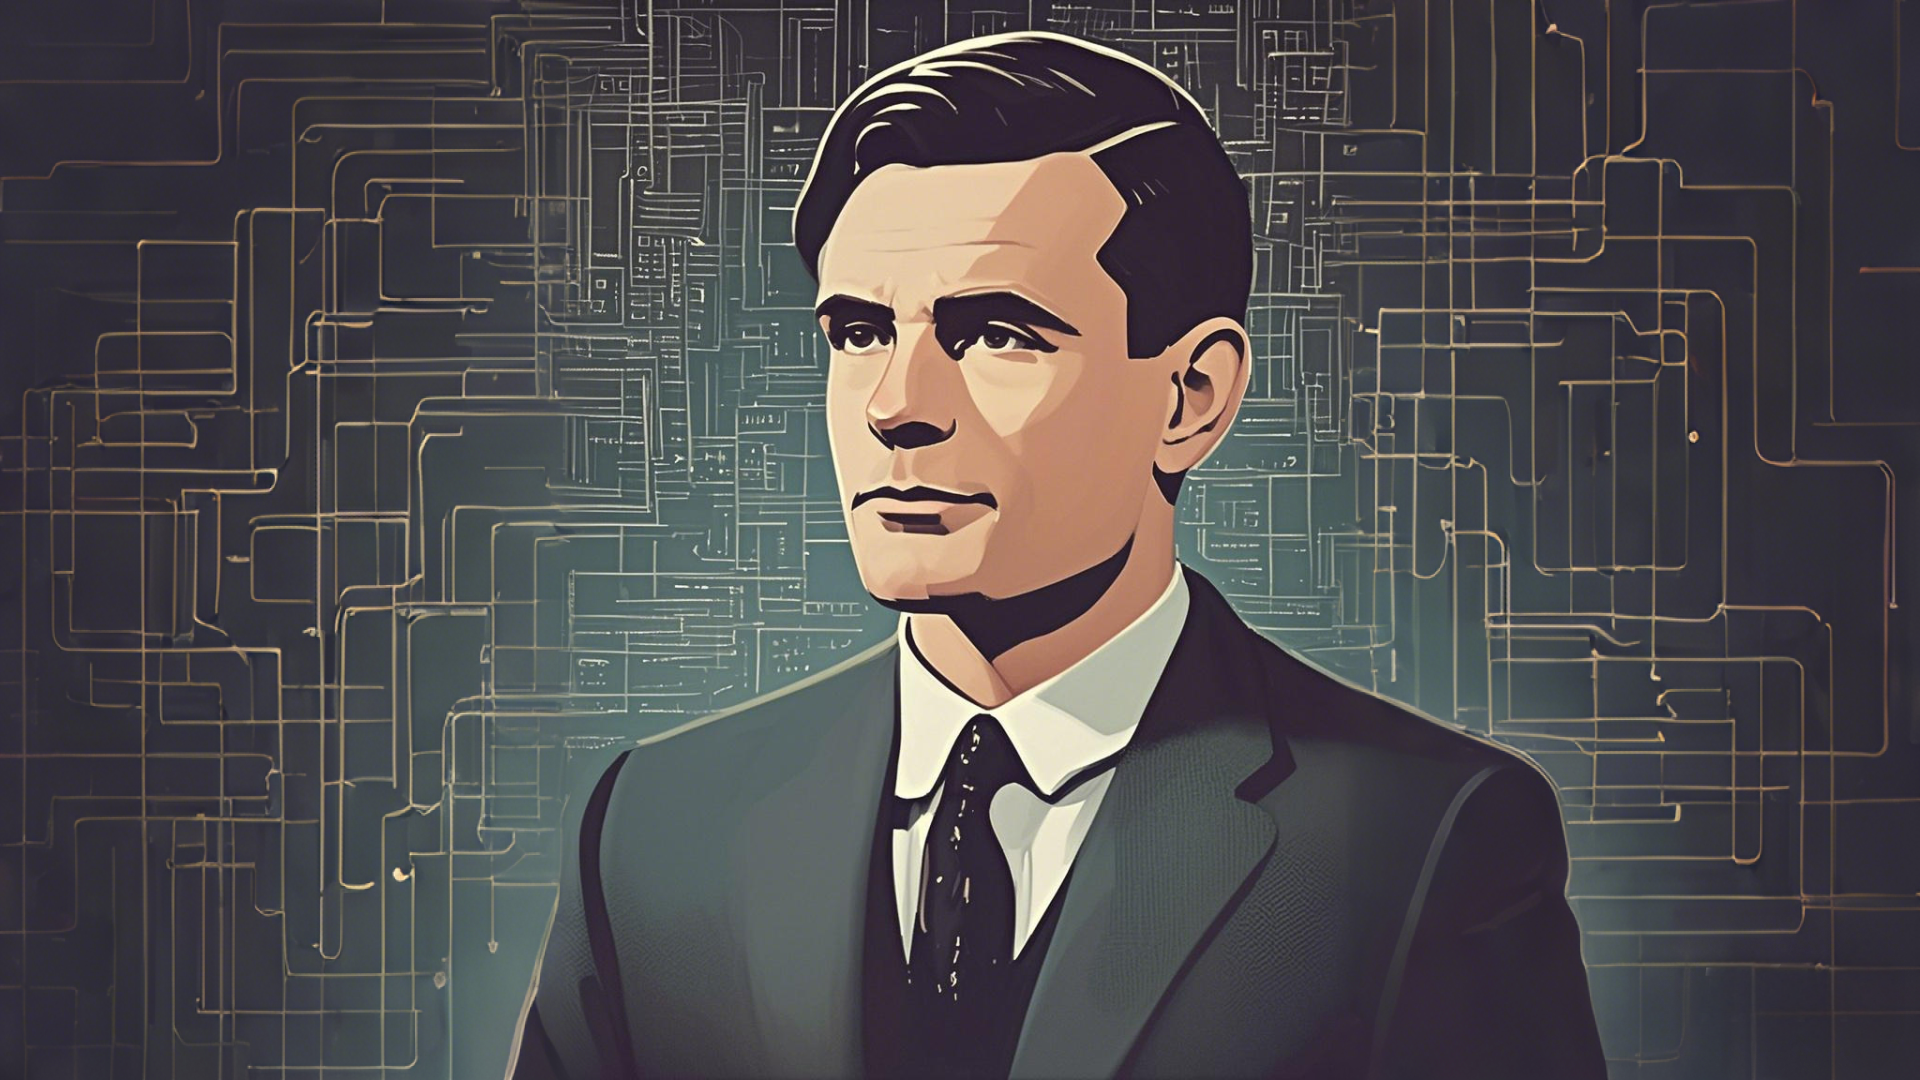
\includegraphics[width=0.75\linewidth]{image/1/Turing.png}
    \caption{“计算机科学之父”艾伦图灵 (图片由 AI 生成)}
\end{figure}
%艾伦・图灵人物小传:1912 年 6 月 23 日出生于英国伦敦,是一位极具影响力的科学家。他在 1936 年提出了 “图灵机” 这一抽象计算模型,为现代计算机的发展奠定了理论基础,被后人称为 “计算机科学之父”。
%二战期间,图灵加入英国密码破译机构,成功设计 “图灵炸弹” 装置,破解德军恩尼格玛密码机,为盟军胜利做出巨大贡献。1950 年,他发表论文《计算机器与智能》,首次提出 “人工智能” 概念,并提出 “图灵测试”,虽有局限性,但启发了关于机器智能的广泛讨论,因此被誉为 “人工智能之父”。
%图灵的贡献推动了计算机科学从理论研究走向实践应用,其成果广泛应用于多个领域。他的思想和理论激励着后来的研究者不断探索创新,对科技界乃至人类社会产生了深远影响。
%然而,由于当时社会对同性恋的偏见,图灵遭受不公正对待,1954 年选择结束自己的生命。但他的科学遗产和对后世的影响不容置疑,其故事也促使人们反思社会的包容性。


在这个游戏场景中,主要涉及三方:询问者、被测试的机器和作为对照的人类。询问者通过书面形式向机器和人类提出各类问题,然后依据他们的回答来判断谁是机器谁是人类。如果在经过充分的询问和交流后,询问者无法准确地分辨出机器和人类的身份,那么就可以认为这台机器通过了图灵测试,展现出了类似人类的智能。由于图灵对人工智能和计算机科学领域开创性的贡献,后人将这种评估人工智能系统智能程度的测试方法称之为“图灵测试”。尽管图灵预测50年后(也即2000年)可能会出现在模仿游戏中表现出色的计算机,使得平均询问者难以准确区分机器和人类,但至今为止,还没有确凿的证据表明存在完全通过图灵测试的机器。
\begin{figure}[htb]
	\centering
	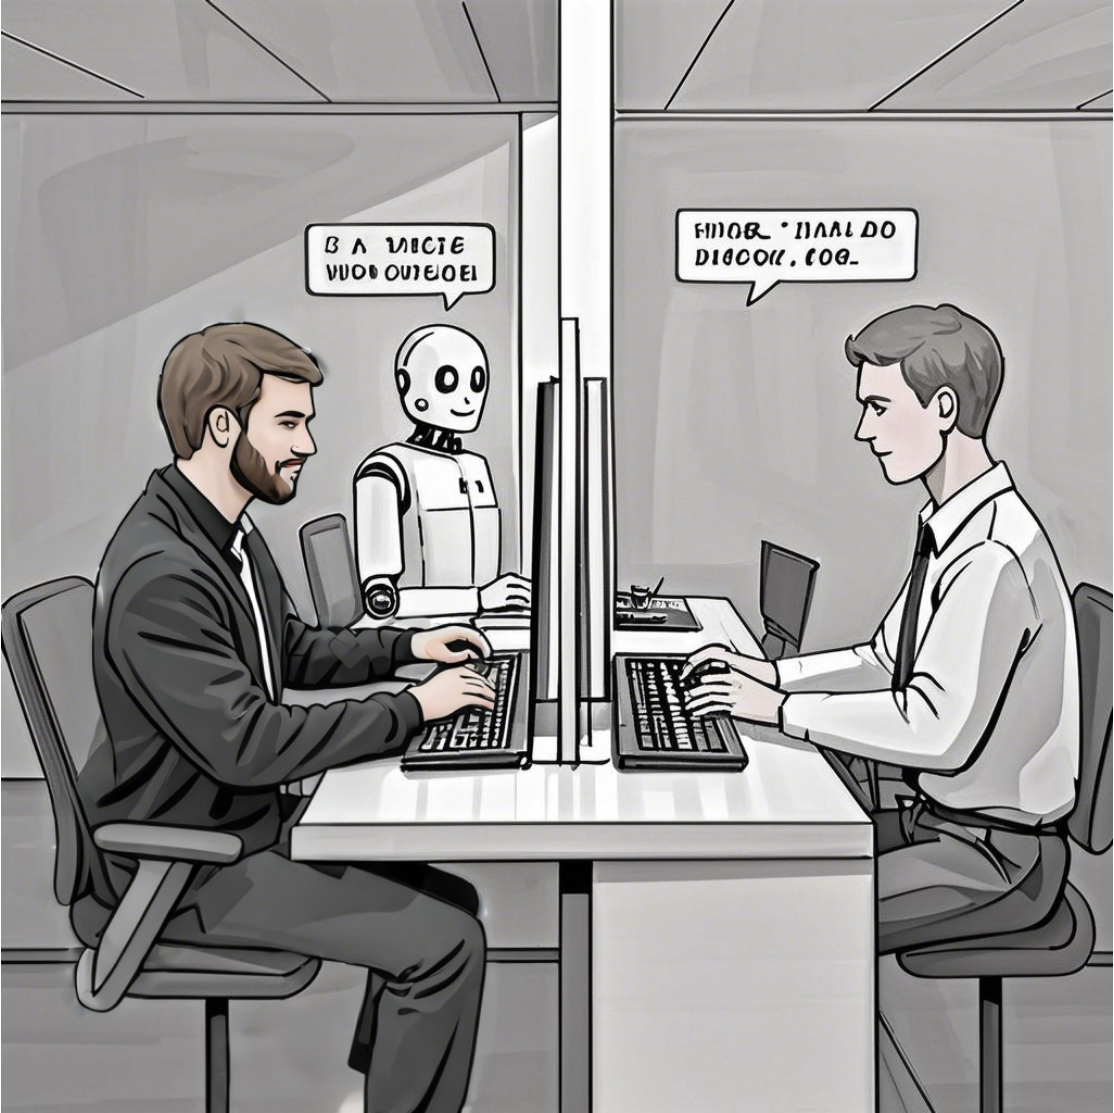
\includegraphics[width=0.75\linewidth]{image/1/图灵测试1.png}
	\caption{图灵测试 (图片由 AI 生成)}
\end{figure}

艾伦·图灵在《计算机器与智能》这篇文章中不仅提出了模仿游戏的概念,还提出了“机器具备思考能力”的论点,并且驳斥了当时几个主流的关于“机器不能思考”的观点。首先,当时的神学观点认为思考是人类不朽灵魂的功能,上帝只赋予人类灵魂,动物和机器没有,所以机器不能思考。而“鸵鸟” 观点(因为和“把头埋在沙子”的“鸵鸟行为”类似而得名),则观点认为机器思考的后果可怕,希望机器不能思考。还有数学观点认为数学逻辑的一些结果表明离散状态机存在局限性,如哥德尔定理等。意识观点认为只有机器能像人类一样因思想和情感创作(如写十四行诗、作曲等)并感知自身行为,才能认为机器有思考能力。各种能力缺失观点则列举了机器无法具备的多种能力,如善良、有幽默感、谈恋爱等。洛夫莱斯夫人(Lady Lovelace)提出分析机只能按人类指令执行,不能创新。\footnote{洛夫莱斯夫人(Lady Lovelace):原名奥古斯塔·艾达·拜伦,是英国浪漫主义诗人拜伦勋爵和妻子安娜贝拉·米尔班克的唯一婚生女,她出生五周后,父母就因为感情不和而分居,母亲带着她离开了父亲,由于母亲出身贵族且热爱数学和天文学,于是从小让她学习逻辑、数学等课程,1833年,艾达结识了数学家查尔斯·巴贝奇,她编写了首个计算机程序,她创建的循环和子程序等概念是现代编程重要基础,确立了编程在计算机系统的核心地位,推动软件发展。她还拓展了计算机功能认知,预见计算机通用性,打破当时狭隘认知,为多领域应用奠基,其思想也启发了人工智能探索,为该领域发展播下种子。}神经系统连续性观点认为神经系统不是离散状态机,离散状态机无法模拟其行为。行为不规范性观点认为人类行为没有固定规则,而机器需按规则运行,所以人类不是机器。超感官知觉观点则提出超感官知觉现象与科学观念冲突,可能影响模仿游戏结果。
\begin{figure}[htb]
    \centering
    
\includegraphics[width=0.75\linewidth]{image/1/lovelance.png}
    \caption{“第一位程序员”艾达洛夫莱斯 (图片由 AI 生成)}
\end{figure}


对于以上观点,图灵都对此进行了逐一反驳,对于神学观点,图灵认为此观点缺乏说服力,且限制了上帝的全能性,认为构造思考机器如同人类生育一样,是上帝意志的体现,同时神学论证在过去常被证明是不令人满意的。对于鸵鸟观点,图灵认为此观点不具实质性,无需反驳,更像是一种情感上的担忧而非理性论证。对于数学观点,他承认特定机器有局限性,但指出没有证据表明人类智能不存在类似局限,人类也常给出错误答案,不能因机器在某些问题上的局限性就认为其不能思考。
图灵认为意识观点极端且类似唯我论,若机器能在模仿游戏中像人类一样回答问题,应可被视为具有思考能力,意识的奥秘不一定要在回答机器能否思考问题前解决。
图灵认为这些观点大多基于不科学的归纳,许多能力与存储容量有关,且机器可以通过编程在一定程度上模拟这些能力,如故意犯错、以自身行为为思考对象等,部分观点是意识观点的变相表达。
图灵指出如果有能创新的离散状态机,分析机在存储和速度足够时可模拟它,且机器常做出让人意外的事,“机器不能创新” 观点可能源于哲学家和数学家的错误假设。
对于,图灵通过与微分分析仪类比,说明在模仿游戏条件下,询问者难以区分数字计算机和连续机器,所以此观点不影响对机器思考能力的探讨。
图灵指出行为不规范性观点的论证存在逻辑问题,且虽然人类行为看似无规则,但科学观察也难以发现完整的行为规律,即使对于简单程序,也难以预测其所有行为。
对于超感官知觉的观点,图灵认为若承认超感官知觉,需加强测试条件,如将参与者置于 “防心灵感应房间”,以确保测试准确性。


图灵测试虽然在人工智能发展历程中有着举足轻重的地位,为衡量机器智能提供了一种开创性的思路,但它也存在很多缺点。一方面,图灵测试高度依赖于语言交流,仅仅聚焦于文本对话场景,忽视了智能体在现实世界中诸多其他重要的智能表现形式,如视觉感知、运动控制等能力。这就好比仅通过一场书面问答来评判一个人的综合能力,显然是片面的。另一方面,测试结果具有较强的主观性,评判者的个人知识储备、思维方式乃至情绪状态等因素都会干扰最终判断,不同评判者对同一机器的评判可能大相径庭。而且,一些机器通过巧妙设计的固定话术套路,可能在短期内 “骗过” 评判者,却并非真正具备理解和思考能力。鉴于图灵测试的这些局限性,人们开始探寻其他途径来深入探讨机器智能的本质,这就引出了另一个极具影响力的思想实验 —— 中文屋思想实验,它从新的角度对机器能否拥有真正的智能发起了挑战。


\textbf{2、中文屋子思想实验}


由约翰西塞尔\footnote{约翰・西塞尔(John Searle),1932 年 7 月 31 日出生于美国科罗拉多州丹佛市。青年时期赴牛津大学求学,在此期间深入研读哲学与语言学经典,与罗素、奥斯汀等知名学者交流,积累了深厚的学术素养,为后续学术发展打下基础。学业完成后,西塞尔就职于加州大学伯克利分校,投身教育多年,开设了 “当代心灵哲学前沿问题探究”“语言逻辑与意义构建” 等课程,培养出众多哲学及相关领域人才。在学术研究方面,他成果丰硕,著作众多。早期的《语言与社会现实》,深入探讨语言在构建社会关系、反映社会结构上的作用,为跨学科语言研究提供新思路;中期著作《意识的结构与功能》,结合哲学思辨与科学认知,剖析人类意识的内在构成及其在认知、行为驱动方面的功能,引发学界对意识本质的广泛探讨;晚年的《哲学反思:跨越边界的洞察》,整合其一生学术成果,跨越心灵、语言、社会等多领域,呈现出综合性的哲学视野,对当代哲学及相关学科发展具有重要推动作用。}于1980年在他的著作《思想,大脑,程序》(Minds, Brains, and Programs)中提出。
实验假设了一个封闭的房间,里面有一个只会说英语的人(塞尔本人常被用来举例),他手头有一本详细的规则手册(用英文书写)。房间外有人通过一个缝隙向房间内传递写有中文问题的纸条。
房间里的人虽然不懂中文,但可以根据规则手册中的指令,对传入的中文问题进行处理。他通过识别中文符号的形状,按照规则手册中规定的操作步骤,对这些符号进行转换和组合,然后将生成的中文回答写在纸条上,再通过缝隙传出房间。从房间外的观察者来看,房间似乎能够理解中文问题并给出合理的回答,因为每次都能得到看似正确的回应。然而,房间内的人实际上对中文一无所知,他只是机械地按照规则进行操作,并不理解问题和答案的含义。

\begin{figure}[htb]
	\centering
	
\includegraphics[width=0.75\linewidth]{image/1/中文屋.png}
	\caption{中文屋子思想实验 (图片由 AI 生成)}
\end{figure}

中文屋子的实验引发了对于计算机是否真正 “理解” 语言的思考。如果计算机仅仅是按照程序规则处理符号,就像房间里的人处理中文一样,那么它是否真的理解了所处理的信息呢?除此之外,“中文屋子” 思想实验挑战了图灵测试等将行为表现等同于理解和智能的观点。它表明,即使一个系统能够在外部表现出看似理解语言的行为,但内部可能并没有真正的理解或意识发生。这使得人们重新审视人工智能的定义和发展方向,思考智能的本质是否仅仅可以通过符号处理和算法来实现,还是需要涉及到真正的语义理解、意识和主观体验等更深层次的因素。

\section{人工智能发展历史}


% 在科技的浩瀚星空中,人工智能宛如一颗最为璀璨且神秘的星辰,其发展历程犹如一部波澜壮阔的史诗,不断书写着人类智慧与创新的传奇。从最初的萌芽到如今的蓬勃兴起,每一个阶段都凝聚着无数先驱者的心血与梦想,深刻地改变着我们的生活与社会的方方面面。回溯人工智能的发展轨迹时,便如同踏上了一段穿越时空的奇妙之旅,见证着那些具有里程碑意义的突破与变革。


自诞生之日起,人工智能就以一种势不可挡的姿态,逐渐渗透到各个领域。它起始于简单的逻辑推理与数学运算的探索,而后在计算机技术的强力推动下茁壮成长。历经岁月的洗礼,人工智能在模式识别、自然语言处理、机器学习等关键领域不断取得令人瞩目的成就,从实验室的理论研究逐步迈向现实世界的广泛应用,成为推动现代社会发展的核心力量之一,而这一切的背后,是一段段充满挑战与机遇的奋斗故事。


\subsection{人工智能的第一个热潮}


在 20 世纪 50 - 70 年代,人工智能迎来了发展史上的第一个热潮。彼时,以美国为例,众多高校纷纷设立人工智能实验室,吸引了大量科研人才投身其中。像斯坦福人工智能实验室,自 1962 年建立后,迅速成为人工智能领域集研究、教育、理论探讨与实践的科研中心,汇集了计算机视觉、机器人技术、机器学习等诸多领域的专家学者,不同专业背景的人才相互协作,探索人工智能的无限可能,呈现出门庭若市的繁荣景象。再如麻省理工学院,其相关科研项目广泛涉及图像处理、机器人研发等多个前沿方向,研究成果频出,让人们对人工智能的未来满怀憧憬。


前文讲到的图灵测试的概念,则为后续计算机科学的发展奠定了坚实的理论基石,其抽象的计算模型为理解计算机的本质和能力边界提供了关键的理论工具,也为人工智能的研究指明了方向,提供了重要的思想基础,成为了后世无数计算机科学家和人工智能研究者灵感的源泉。


在这一时期,除了艾伦・图灵的卓越贡献外,还有其他一些理论也对人工智能的理论体系产生了深刻影响。例如,沃伦・麦卡洛克(Warren McCulloch)\footnote{沃伦・麦卡洛克(Warren McCulloch):美国神经学家,计算神经科学的开创者之一。他与沃尔特・皮茨于 1943 年首次提出类似系统,对神经网络领域的发展影响深远。}和沃尔特・皮茨(Walter Pitts)\footnote{沃尔特・皮茨(Walter Pitts):美国数学家,12 岁时阅读罗素著作并挑出错误,后得到罗素赏识。他与沃伦・麦卡洛克合作提出 “麦卡洛克 — 皮茨模型”(简称 M-P 模型),该模型是神经网络领域的开山之作,将神经元描述成一个逻辑门,通过对周边神经元信号加权求和等操作来模拟脑神经活动,为后续深度学习技术奠定了基础。}在 1943 年提出的神经元模型,将神经元的工作原理抽象为数学逻辑形式,为人工神经网络的发展奠定了基础,启发了研究者们对大脑神经元结构与智能之间关系的深入思考,使得模拟人类大脑的神经网络成为人工智能研究的重要方向之一。他们的理论为后来者构建能够学习和处理复杂信息的人工神经网络提供了关键的理论支撑,推动了人工智能在模仿人类智能学习和认知过程方面的探索。此外,克劳德・香农(Claude Shannon)\footnote{克劳德・香农(Claude Shannon):美国著名数学家、发明家、密码学家,被誉为 “信息论之父”。他于 1948 年发表了具有划时代意义的《通信的数学理论》,在该论著中系统性地阐述了信息论,提出众多开创性概念与理论,其中就包括信息熵。香农的研究成果为现代通信技术、计算机科学以及人工智能等诸多领域奠定了坚实的理论根基,彻底改变了人们对信息传输、存储与处理的认知方式。例如,他通过引入比特这一概念,将信息量化,让信息能够如同实体物品般被精准度量、操控,极大推动了数字通信时代的到来,为人类迈入信息社会铺就了道路。}于 1948 年发表的《通信的数学理论》,引入了信息熵\footnote{信息熵:由克劳德・香农提出的一个核心概念,用于量化信息的不确定性程度。在信息传输过程中,熵值越高,意味着信息的不确定性越大,所蕴含的信息量也就越丰富。从数学角度,它以特定的公式进行计算,该公式基于信息源发出不同符号的概率分布。打个比方,在天气预报场景中,如果天气预报员说 “明天要么晴天要么雨天”,这种高度不确定的表述所携带的信息熵就相对较高;而若说 “明天肯定是晴天”,几乎没有不确定性,信息熵则趋近于零。信息熵这一概念为数据压缩、信道编码等信息处理技术提供了关键的理论指引,确保信息能够高效、精准地传输与存储,在人工智能的数据处理环节,它帮助机器理解数据中的信息量大小,从而合理分配计算资源,更高效地从海量数据中挖掘有价值的知识。}的概念,让研究者们开始思考如何优化信息的传输、存储和处理,以提高智能系统的效率和性能,这一理论在人工智能的数据处理和决策优化等方面具有重要的指导意义,促进了人工智能理论体系在信息处理维度的完善和发展,共同为 1956 年人工智能作为一门独立学科的诞生积累了丰富的理论养分,营造了浓厚的学术氛围。


1956 年夏季,在美国新罕布什尔州汉诺威镇的达特茅斯学院召开的达特茅斯会议,是人工智能发展史上的关键转折点,具有不可磨灭的标志性意义,被视为这一领域的重要里程碑。此次会议由约翰・麦卡锡、马文・明斯基(Marvin Minsky)\footnote{马文・明斯基(Marvin Minsky):美国认知科学家,早期人工智能的代表性人物。与艾伦・纽厄尔、赫伯特・西蒙等一同引领符号主义学说在人工智能领域占据统治地位长达半个多世纪。他在知识表示、机器人学等方面贡献突出,提出了框架理论,试图为计算机理解和表示知识提供一种结构化的方法,推动机器像人类一样认识和理解世界。}与艾伦・纽厄尔\footnote{艾伦・纽厄尔(Allen Newell):美国计算机科学家,与赫伯特・西蒙合作,在人工智能的早期发展中提出诸多有影响力的理论和方法。二人共同开发了第一个启发式程序 “逻辑理论家”,它能够模拟人类的逻辑推理过程,证明数学定理,为人工智能的逻辑推理和问题解决能力发展作出开创性贡献,同属符号主义学派代表人物}、赫伯特・西蒙(Herbert Simon)\footnote{赫伯特・西蒙(Herbert Simon):美国经济学家、计算机科学家,和艾伦・纽厄尔紧密合作,在符号主义人工智能发展进程中扮演关键角色。他在决策理论、管理科学等多领域造诣深厚,凭借其在人工智能等多方面成就荣获诺贝尔经济学奖。他提出的有限理性理论,应用于智能决策系统,使机器在复杂环境下能做出更合理决策,其研究成果广泛应用于智能系统的构建。}等一同引领符号主义学说在人工智能领域占据统治地位长达半个多世纪,对人工智能的理论、技术发展尤其是在知识表示、机器人学等方面贡献突出。克劳德・香农(Claude Shannon)和纳撒尼尔・罗切斯特(Nathaniel Rochester)\footnote{纳撒尼尔・罗切斯特(Nathaniel Rochester):美国科学家,早期参与人工智能相关研究,在该领域发展初期发挥了一定作用,推动了一些早期探索性项目的开展,比如参与早期计算机系统与人工智能算法结合的实践,为后续研究积累了宝贵经验。}四人牵头发起并负责筹备组织工作。他们凭借自身在学术界和科研领域的影响力与号召力,吸引了来自多个不同领域的十余名顶尖专家学者。这些领域涵盖数学、计算机科学、神经心理学\footnote{神经心理学:作为心理学的一个分支,主要研究神经系统特别是大脑与心理过程之间的关系,为人工智能模拟人类大脑功能、理解认知机制等提供了理论基础。各国神经心理学家通过大量实验,揭示大脑神经活动与感知、记忆、思维等心理现象的关联,助力人工智能研究者从神经科学角度探索智能的本质。}、认知心理学\footnote{认知心理学:致力于研究人的高级心理过程,如认知、思维、记忆、语言等。其研究成果有助于人工智能系统模拟人类的认知模式,各国学者提出的诸多认知模型和理论,使机器在感知、理解、决策等方面更接近人类智能,比如瑞士心理学家皮亚杰的认知发展理论对人工智能教育应用领域有重要启发。}以及信息论\footnote{信息论:由美国数学家克劳德・香农创立,主要研究信息的量化、存储、传输等问题。他 1948 年发表的《通信的数学理论》具有划时代意义,提出信息熵的概念以及数学表达式,推出比特的概念,为现代信息论奠基,也为人工智能中的数据处理、通信、知识表示等多个环节提供了关键理论支撑,让机器能够高效处理和传输信息。}等,参会人员均在各自专业领域拥有深厚造诣和丰富经验,代表了当时科学界在相关领域的前沿水平。
\begin{figure}[htbp]
    \centering
    
\includegraphics[width=0.75\linewidth]{image/1/John McCarthy.png}
    \caption{“人工智能之父”约翰麦卡锡 (图片由 AI 生成)}
\end{figure}

会议进程中,专家学者们围绕智能机器的理论与实践展开了深入且细致的探讨与交流。在经过多轮严谨的论证和思维碰撞后,首次明确提出了 “人工智能” 这一术语,这不仅仅是一个名称的确定,更是对一个全新研究领域的精准定位。他们从学术层面深入剖析了人工智能所涉及的理论体系,包括但不限于逻辑推理、知识表示、机器学习等核心理论分支,并详细规划了这些理论在实际应用中的方向和场景,如工业自动化生产中的智能控制系统、医疗诊断领域的辅助决策系统以及交通运输中的智能调度系统等,清晰界定了其研究范畴。同时,确立了人工智能的发展目标,旨在创造出能够模拟人类智能行为,甚至在某些特定任务上超越人类智能的机器系统,通过构建基础理论框架,为后续的研究工作提供了系统性的指导原则和方法路径。这一系列成果标志着人工智能成功摆脱萌芽期的混沌无序状态,正式作为一门独立学科登上了科学技术的历史舞台,引发了科学界、产业界以及社会各界对这一新兴领域的广泛关注和探索热情,从而拉开了人工智能第一个热潮的序幕。


在这一发展阶段,符号主义成为人工智能研究的主流方向。在此理论框架下,研究工作取得了多项具有开创性的初步成果。艾伦・纽厄尔(Allen Newell)\footnote{艾伦・纽厄尔(Allen Newell):美国计算机科学家,与赫伯特・西蒙合作,在人工智能的早期发展中提出诸多有影响力的理论和方法。二人共同开发了第一个启发式程序 “逻辑理论家”,它能够模拟人类的逻辑推理过程,证明数学定理,为人工智能的逻辑推理和问题解决能力发展作出开创性贡献,同属符号主义学派代表人物。}和赫伯特・西蒙(Herbert Simon)\footnote{赫伯特・西蒙(Herbert Simon):美国经济学家、计算机科学家,和艾伦・纽厄尔紧密合作,在符号主义人工智能发展进程中扮演关键角色。他在决策理论、管理科学等多领域造诣深厚,凭借其在人工智能等多方面成就荣获诺贝尔经济学奖。他提出的有限理性理论,应用于智能决策系统,使机器在复杂环境下能做出更合理决策,其研究成果广泛应用于智能系统的构建。}开发的逻辑理论家,作为人工智能早期的重要成果之一,能够运用逻辑推理规则对数学定理进行证明,这在当时展示了计算机在处理复杂逻辑问题上的潜力,为后续更高级的智能推理系统开发提供了重要的技术思路和方法借鉴。通用问题求解器的出现则进一步引入了启发式搜索\footnote{启发式搜索:一种人工智能搜索策略,它不像传统的盲目搜索遍历所有可能,而是利用经验法则、启发信息来引导搜索方向,优先探索更有可能通向目标解的路径,大大提高了搜索效率,广泛应用于路径规划、问题求解等诸多领域,不同国家科研团队基于不同应用场景对其进行优化拓展。}概念,通过对问题空间的智能搜索策略,提高了计算机解决复杂问题的效率和能力,使得人工智能在逻辑推理与问题解决方面向实用化迈进了重要一步。


在语言处理领域,早期机器翻译研究也开始起步。尽管受到当时技术条件的诸多限制,如语言规则的复杂性、词汇语义的多样性以及不同语言文化背景差异等因素影响,翻译成果的准确性和流畅性有限,但这一探索为后续机器翻译技术的发展积累了宝贵的实践经验,包括语言数据的收集与整理方法、语法和语义分析模型的构建思路以及翻译算法的优化方向等。


约瑟夫・魏泽鲍姆\footnote{约瑟夫・魏泽鲍姆(Joseph Weizenbaum):德国计算机科学家,开发了 ELIZA 程序。他通过这一程序揭示了人工智能可能带来的社会影响,让人们意识到机器与人交流背后的伦理问题,激发了全球范围内对人工智能伦理规范、人机关系界定的探讨,推动该领域向更注重人文关怀方向发展。}开发的 ELIZA 程序在自然语言处理与人机对话技术方面取得了初步进展,该程序能够模拟简单的对话场景,对用户输入的自然语言文本进行一定程度的理解和回应,虽然其对话能力还较为初级,但为后续更加智能和复杂的人机对话系统开发奠定了基础。


与此同时,计算机在其他领域也展现出了初步的智能应用能力,例如能够解决代数应用题,通过对数学问题的理解和算法运算得出正确答案;能够证明几何定理,运用几何知识和推理规则完成定理的证明过程;还能够学习和使用英语,包括词汇的记忆、语法的运用以及简单文本的理解和生成等功能,这些成果在当时极大地激发了人们对人工智能未来发展的想象空间。


1965 年,爱德华・费根鲍姆(Edward Feigenbaum)成功开发出首个专家系统 DENDRAL,这一成果在人工智能的发展进程中具有重要的标志性意义。DENDRAL 系统专注于化学领域,通过整合该领域丰富的专业知识和大量的实践经验,构建了完善的知识库和高效的推理机制,能够有效地模拟人类专家在分子结构鉴定方面的决策过程。具体而言,它能够依据质谱数据所提供的分子碎片信息,运用知识库中的化学知识和推理规则,准确推断出分子的结构组成,这一应用极大地提高了化学研究中分子结构鉴定的效率和准确性,为后续专家系统在各个不同专业领域的广泛开发和应用提供了成功范例和技术基础,推动了专家系统这一重要人工智能分支的蓬勃发展。


同样在这一时期,1957 年弗兰克・罗森布拉特Frank Rosenblatt)\footnote{弗兰克・罗森布拉特(Frank Rosenblatt):美国心理学家,发明了感知机,这是一种早期的人工神经网络模型,为神经网络的后续发展开启了道路,尽管初期感知机存在一定局限性,但为深度学习等后续技术演进提供了重要起点。:发明了感知机,这是一种早期的人工神经网络模型,为神经网络的后续发展开启了道路,尽管初期感知机存在一定局限性,但为深度学习等后续技术演进提供了重要起点。}发明的感知机作为早期神经网络模型的重要代表,为机器学习和人工智能的长远发展提供了关键的基础支撑。感知机模型基于神经元的基本结构和工作原理,通过对输入数据的加权处理和阈值判断,实现对简单模式的识别和分类功能,为后续神经网络技术的发展提供了最初的理论和实践模型。


1959 年,亚瑟・萨缪尔(Arthur Samuel)\footnote{亚瑟・萨缪尔(Arthur Samuel):美国计算机科学家,被认为是提出机器学习概念的先驱之一,他在 20 世纪 50 年代将机器学习应用于西洋跳棋程序,使程序能够自我学习提高棋艺,开创了机器学习在实际应用中让机器自主提升性能的先河。}提出 “机器学习” 这一具有深远影响的术语,并通过开发会下跳棋的计算机程序对该概念进行了成功验证。这个程序创新性地采用自学习策略,基于 “启发式搜索” 不断优化下棋决策过程。在与跳棋冠军的实际对弈中,通过不断学习和改进自身的下棋策略,展现出超越普通玩家的水平,这一成果充分证明了计算机通过学习能够提升自身智能水平的可能性,为机器学习领域的后续发展指明了方向。


然而,任何技术的发展都受时代背景与技术条件的制约,人工智能的早期发展便是如此。在人工智能发展初期,计算能力和数据量成为了关键瓶颈。彼时,计算机运算速度与存储容量有限,难以满足复杂算法对大量数据的处理和快速运算需求。例如在复杂图像识别领域,由于计算力不足,面对高分辨率图像的海量像素信息,系统难以快速、精准地提取特征和识别模式,图像识别的准确率与速度远未达到实际应用标准。在自然语言语义理解方面,受限于缺乏大规模语料库数据支撑,以及计算能力的掣肘,计算机仅能理解简单语句结构与字面意思,对复杂语义关系、隐喻、歧义等语言现象处理能力不足,导致进展缓慢。这使得早期许多人工智能方法在处理实际复杂问题时困难重重,难以实现预期效果。


随着时间的推移,成果转化的困境逐渐显现。以美国一些高校的人工智能实验室为例,尽管前期投入了大量人力、物力,但由于技术瓶颈,研发成果难以落地转化为实用产品,无法产生经济效益。经费紧张的压力随之而来,实验室不得不缩减规模,甚至关停部分项目。同时,政府与投资方的热情也逐渐消退。美国国防部高级研究计划局(DARPA)在持续投入多年却未见显著成效后,大幅削减了对人工智能领域的资金投入。20 世纪 70 年代,其资金投入占比持续下降。英国等其他国家政府也相继停止拨款。多重因素的共同作用下,人工智能的第一个热潮在 70 年代逐渐消退,步入了发展的寒冬期。


尽管如此,这一时期的研究成果依然在人工智能的发展长河中具有不可忽视的重要地位。这些早期的探索和实践为后续人工智能的发展积累了丰富而宝贵的经验和教训,无论是成功的技术思路和方法,还是失败的尝试和遇到的问题,都为后来的研究者提供了重要的参考依据和借鉴方向。这些成果奠定了人工智能发展的坚实基础,在学术理论、技术实践以及人才培养等多个方面都产生了深远的影响,引导着后续研究在曲折中不断前行,朝着更加深入、更加有效的方向持续发展,为人工智能在未来的突破和腾飞积蓄了力量。



\subsection{人工智能的第二个热潮}


20 世纪 80 年代至 90 年代,人工智能迎来了第二次热潮,其中专家系统的兴起成为主要驱动力之一。专家系统聚焦于特定领域知识的精准表示与严密推理,核心在于精心构建知识库和推理引擎。


在医疗诊断领域,它能依据大量医学知识和临床经验,综合分析患者症状、检查结果等信息,辅助医生做出更准确诊断;在化学分析方面,卡耐基梅隆大学为美国数字设备公司开发的专家系统 xcom,7 年间为该公司节约了 4000 万美元,它能有效解读化学数据,优化生产流程。这一显著经济效益引发了全球开发和部署专家系统的浪潮。


与此同时,语音识别技术也取得重要突破。研究人员摒弃符号学派传统思路,采用统计思路解决实际问题。通过对大量语音数据的统计分析,语音识别系统能更好应对语音变化和不确定性,精准识别语音内容,大幅提升准确率和实用性。例如,在语言交互场景中,系统能够更准确识别用户命令,为智能语音交互发展奠定基础,智能语音助手等应用开始出现。


然而,专家系统虽在特定领域成功,但也暴露出诸多问题。知识获取需耗费大量人力、物力和时间,依赖领域专家经验,效率低下;随着知识更新和领域变化,知识库维护复杂且成本高昂;面对复杂现实情况,其处理不确定性问题能力有限,推理能力受制约。这些问题致使专家系统应用范围受限,优势减弱,人工智能研究再次陷入低谷。


在这一时期,众多重要人物及其研究成果为人工智能的发展添砖加瓦。1975 年马文・明斯基提出框架理论用于知识表示,1976 年大卫・马尔提出视觉计算理论并由学生归纳总结成书。1976 年兰德尔・戴维斯发表文章提出提高知识库开发、维护和使用完整性的方法。1979 年卡耐基梅隆大学为 DEC 公司制造的专家系统可节约大量费用。1980 年德鲁・麦狄蒙和乔恩・多伊尔提出非单调逻辑。罗德尼・布鲁克斯(Rodney Brooks)\footnote{罗德尼・布鲁克斯(Rodney Brooks):澳大利亚计算机科学家,倡导基于行为的机器人学,反对传统机器人复杂的中央控制模式,主张让机器人通过简单行为模块的交互实现智能,开发的机器人在实际场景适应性、自主行动能力上表现突出,推动了机器人技术革新,让机器人能更灵活应对现实世界复杂环境。}等人推动了基于行为的机器人学快速发展。


1982年,约翰・霍普菲尔德(John Hopfield)\footnote{约翰・霍普斯菲尔德(John Hopfield):美国物理学家,提出了霍普斯菲尔德网络,这是一种循环神经网络模型,在联想记忆、优化计算等方面有独特优势,为神经网络在复杂信息处理和模式识别等任务中的应用拓宽了道路。}构建了一种新的全互联的神经元网络模型,具有自联想记忆和异联想记忆的功能,为神经网络的发展开辟了新方向, 1982 年发表的论文《视觉计算理论》对认知科学影响深远,其研究成果对认知科学和人工智能领域产生了重要影响。道格拉斯・莱纳特从事机器学习、知识表示等研究,其博士论文《数学中发现的人工智能方法 —— 启发式搜索》描述了名为 “AM” 的程序,该程序能在大量启发式规则的指导下开发新概念数学,为人工智能在知识发现和概念形成方面的研究提供了有益的探索路径。


1985 年,朱迪亚・珀尔(Judea Pearl)\footnote{朱迪亚・珀尔(Judea Pearl):以色列计算机科学家,在人工智能的不确定性推理、因果关系推断等方面做出开创性工作,提出贝叶斯网络等方法,使人工智能系统能够更好地处理不确定性信息,提升推理和决策的准确性,广泛应用于医疗诊断、金融风险评估等领域,帮助机器在复杂多变环境中做出合理判断。}首先提出贝叶斯网络。这些成果共同构成了这一时期人工智能发展的丰富画卷,为后续的研究和应用积累了宝贵的经验和技术基础,尽管经历了起伏,但依然推动着人工智能在曲折中不断前进,探索更加广阔的发展空间。1986年,大卫・鲁梅尔哈特(David Rumelhart)\footnote{大卫・鲁梅尔哈特(David Rumelhart):美国认知心理学家,在神经网络研究领域成果丰硕,对反向传播算法等神经网络关键技术的发展与推广起到了重要推动作用,其工作使得神经网络的训练效率大幅提升,促进了深度学习技术走向成熟。}大力推广 “反传法”,这一方法为神经网络的训练提供了关键钥匙,有效解决了权重调整等核心难题,大幅提升了神经网络的学习效率与准确性,推动着技术大步向前迈进。


期间众多具有深远影响力的大事件和发明照亮了技术发展的前路。1980 年,卡耐基梅隆大学受美国数字设备公司委托,成功开发出专家系统 xcom,这一突破性成果仿若一颗火种,瞬间点燃了全球范围内对专家系统开发的热情。专家系统凭借其独特的知识表示与推理能力,在特定领域展现出卓越的问题解决能力,为企业决策、工业流程优化等诸多场景提供了智能化支持,极大地提升了生产效率与决策科学性。


紧接着,1981 年日本政府豪掷 8.5 亿美元倾力打造第五代计算机计划。这一宏伟计划旨在研发能够像人类一样自如对话、精准翻译、高效处理图片以及深度推理的智能机器,力求突破人机交互与智能处理的重重难关。虽然后期因技术瓶颈、目标过于超前等诸多因素致使该计划未能达成预期,但其展现出的全球对人工智能发展的极高期望,犹如一声激昂号角,鼓舞着各国科研人员勇往直前,持续探索人工智能的无限可能。


1984 年,大百科全书(Cyc)项目震撼登场,其试图将人类社会积累的海量知识完整地装进计算机系统,期望赋予人工智能如同人类般深邃的推理能力,能够依据知识储备灵活应对各种复杂情境。尽管受限于当时的技术条件,完全实现这一宏伟目标困难重重,但该项目无疑激发了科研人员对知识表示、推理算法等关键领域的深入研究热情,催生了一系列创新思维与技术突破,为后续人工智能发展筑牢根基。


此外,还有其他重要人物及其成果。1988年,CMU的汉斯・贝利纳\footnote{汉斯・贝利纳(Hans Berliner):美国计算机科学家,在人工智能的博弈领域,尤其是国际象棋程序开发方面有卓越成就,其开发的程序在棋力上达到较高水平,展现了人工智能在复杂策略游戏中的决策能力和学习潜力,通过算法优化让计算机能在复杂棋局中精准决策、快速学习对手策略。}打造的计算机程序战胜双陆棋世界冠军;兰德・戴维斯(Rand Davis)\footnote{兰德・戴维斯(Rand Davis):美国计算机科学家,在人工智能的知识工程、分布式人工智能等领域有深入研究,致力于构建更高效的知识表示与协作系统,推动人工智能从个体智能向群体智能、分布式智能拓展,为多智能体协同工作、知识共享等应用场景提供理论支撑与技术方案。}在斯坦福大学获得人工智能博士学位后,发表文章提出使用集成的面向对象模型来提高知识库开发、维护和使用的完整性;格瑞・特索罗(Gerry Sussman)\footnote{格瑞・特索罗(Gerry Sussman):美国计算机科学家,在人工智能编程、复杂系统构建等方面成果丰硕。他致力于开发实用工具与系统,有力地推动了人工智能从理论迈向实际应用,其工作为智能系统的工程化实现奠定了坚实基础,在人工智能技术的发展进程中发挥了重要的支撑与促进作用。}打造的自我学习双陆棋程序,为增强学习的发展奠定了基础。




然而,到了 1987 年,科技发展的浪潮涌起新的变化。苹果和 IBM 生产的台式机性能实现了质的飞跃,其强大算力与便捷性迅速超越了 Symbolics 公司生产的昂贵 lisp 机。这一转变使得依赖特定硬件环境、成本高昂的专家系统光环渐暗,市场需求与研发方向开始重新洗牌,促使人工智能领域探索更具普适性、性价比更高的技术路径。


硬件性能瓶颈是导致人工智能热潮褪去的另一个因素。当时计算机硬件虽有发展,但无法满足人工智能算法和数据处理需求,且硬件成本高昂,限制了技术推广应用。市场方面,早期对人工智能过度宣传,公众期望过高,而实际应用效果未达预期,导致公众信心受挫,市场需求下滑。同时,人工智能成果商业化困难,面临技术、商业模式等问题,难以实现盈利,资金投入减少。1991 年,曾备受瞩目的日本第五代计算机计划宣告失败 1993 年,人工智能领域深陷信任危机的泥沼。


尽管前期部分技术承诺未能兑现,应用落地困难,人们对人工智能的发展前景产生了诸多质疑。但困境往往孕育转机,科研人员开始深刻反思传统技术路线,积极尝试强化学习、模仿学习等自下而上的全新学习方式。这些创新方法强调智能体与环境的深度交互,通过不断试错、自主学习来优化决策,为人工智能研究开启了全新方向,推动着技术逐步走出低谷,迈向新的发展阶段,这些都为人工智能第三次热潮埋下了伏笔。



\subsection{人工智能的第三个热潮}


20 世纪 90 年代末至今,人工智能迎来了第三次浪潮,这次浪潮展现出前所未有的活力和影响力,深刻地改变着社会的方方面面,推动人类进入智能时代。


1990 年以来,计算能力的大幅提升和数据量的爆炸式增长成为人工智能发展的重要基石。新型人工智能芯片的不断演进,如 GPU 的广泛应用以及各类专为人工智能优化的芯片架构的出现,结合云计算技术的强大支撑,使得计算机能够处理海量的数据和复杂的计算任务,为大规模神经网络模型的训练提供了坚实的硬件保障,极大地加速了人工智能技术的发展进程。


1998 年,杨立昆(Yann LeCun) \footnote{杨立昆 (Yann LeCun):法国计算机科学家,在深度学习领域尤其是卷积神经网络方面有极高造诣,其研究成果大幅提升了图像识别、计算机视觉等领域的性能,推动了人工智能在视觉感知任务中的广泛应用,引领了深度学习在相关领域的发展潮流,开发的卷积神经网络架构被广泛采用,大幅提高图像分类准确率。}提出的卷积神经网络(Convoluted Neural Network),成为深度学习领域的经典算法之一,在图像识别等领域展现出卓越的性能,为后续深度学习算法的发展和应用奠定了基础。进入 21 世纪,机器学习和深度学习逐渐成为人工智能研究的主流方向,并在各行业中得到了广泛的应用,推动了行业的智能化升级。


2006 年杰弗里・辛顿\footnote{杰弗里・辛顿(Geoffrey Hinton):英国计算机科学家,深度学习领域的领军人物之一,对神经网络架构、训练算法等核心技术有诸多突破性创新,为推动深度学习从理论到大规模应用转化付出诸多努力,培养了大量该领域人才,被誉为 “深度学习教父”,他提出的反向传播改进算法等成果加速了深度学习普及。}发表了《一种深度置信网络的快速学习算法》,与此同时,其他重要的深度学习学术文章也相继问世,在基本理论层面取得了一系列重大突破,掀起了人工神经网络的第三次浪潮,为深度学习的广泛应用和深入发展打开了大门,使得神经网络能够更高效地学习和处理复杂的数据模式,从而在图像识别、语音识别、自然语言处理等多个领域取得了显著的成果和进步。
\begin{figure}[htbp]
    \centering
    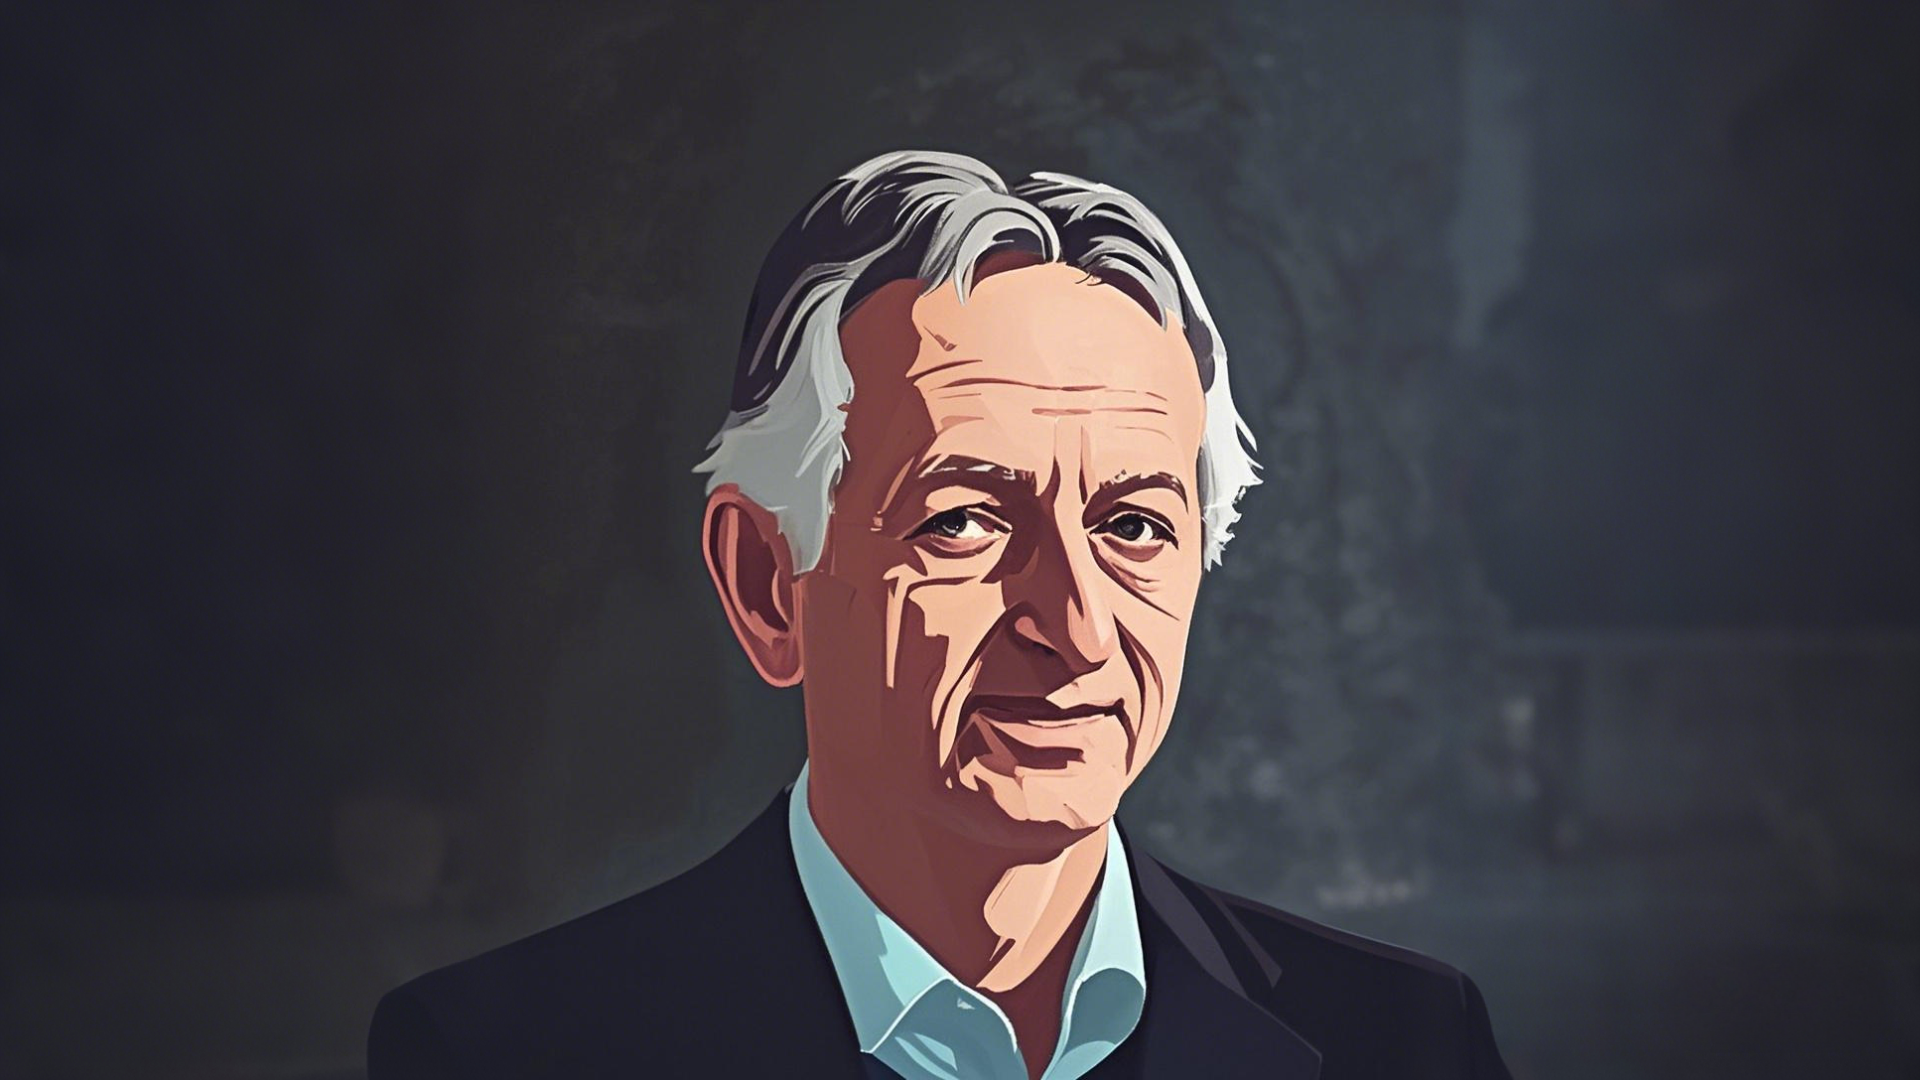
\includegraphics[width=0.75\linewidth]{image/1/Hinton.png}
    \caption{“AI教父”杰弗瑞辛顿 (图片由 AI 生成)}
\end{figure}


互联网的普及和信息技术的飞速发展,催生了海量数据的产生和积累。社交媒体、电子商务、物联网等领域每天都产生着数以亿计的数据,这些丰富多样的数据为人工智能模型的训练提供了充足且多样化的素材。例如,在图像识别领域,大规模的图像数据集如 ImageNet\footnote{ImageNet:由美国斯坦福大学等机构研究人员构建的一个大型的图像数据库,涵盖海量不同类别的图像,为图像识别、计算机视觉领域的研究和算法训练提供了丰富素材,基于 ImageNet 举办的图像识别竞赛极大推动了相关技术快速发展,促使图像识别准确率大幅提升,吸引全球科研团队参与竞争,加速技术突破。} 的出现,使得深度学习模型能够学习到丰富的图像特征,从而在图像分类、目标检测等任务上不断刷新准确率记录;在自然语言处理领域,海量的文本数据让语言模型能够更好地理解和生成人类语言,推动了机器翻译、文本生成、问答系统等应用的发展。


计算能力的提升与数据的增长相辅相成。一方面,强大的计算能力使得数据的处理和分析更加高效,能够快速完成大规模数据的预处理、模型训练和优化;另一方面,丰富的数据又为计算资源的充分利用提供了广阔的空间,促使研究人员不断探索更复杂、更强大的人工智能模型。这种良性循环推动了人工智能技术在各个细分领域的巨大进步,使得人工智能系统的性能和智能水平得到了质的飞跃,能够更好地应对现实世界中的复杂任务和挑战。


近年来,以 ChatGPT 为代表的 AIGC(人工智能生成内容)技术异军突起,成为人工智能领域的又一热点和亮点。AIGC 在内容创作成本、创作效率、模型计算消耗以及用户流量基础等多个维度实现了重大突破。与传统的内容创作方式相比,AIGC 能够利用深度学习模型快速生成高质量的文本、图像、音频、视频等各种类型的内容,大大降低了创作门槛和成本,提高了创作效率,同时也满足了用户日益多样化的内容需求。


AIGC 的应用前景极为广阔,涵盖了搜索引擎、艺术创作、影音游戏、金融、教育、医疗、工业等众多领域。在搜索引擎方面,它能够为用户提供更加精准、个性化的搜索结果和答案,提升搜索体验;在艺术创作领域,帮助艺术家生成创意灵感、辅助绘画、音乐创作等;在影音游戏中,用于生成虚拟角色、场景、剧情等,增强游戏和影视作品的吸引力和沉浸感;在金融领域,辅助风险评估、投资决策等;在教育领域,实现个性化教学、智能辅导等;在医疗领域,辅助疾病诊断、药物研发等;在工业领域,优化生产流程、进行质量检测等。AIGC 的兴起有望大幅加速 AI 的商业化进程,为各行业带来新的增长点和创新机遇,推动整个社会经济的发展和变革。


在这一次人工智能浪潮之下,也有很多研究学者做出了巨大贡献,他们的研究成果与创新实践成为推动人工智能迅猛发展的关键力量,在全球范围内产生了深远的学术与产业影响。杰弗里・辛顿,作为 “AI 教父”“深度学习之父”,其学术生涯成就斐然。早在 1977 年博士论文中对视觉系统假设处理方法的研究,便为计算机视觉和模式识别奠定理论根基,引领该领域新方向。后续在 1998 年当选英国皇家学会会士,2006 年提出深度信念网络,2012 年取得计算机视觉突破性成果,以及 2018 年荣获图灵奖和 2024 年斩获诺贝尔物理学奖等一系列荣誉,彰显了他在深度学习理论与应用上的卓越贡献,深刻影响着全球人工智能的发展轨迹,其研究成果堪称行业标杆。Yann LeCun(杨立昆) 同样贡献卓越,在深度学习和神经网络领域建树颇丰。自 1983 年获得巴黎 ESIEe 电气工程师文凭后持续深耕,1987 年取得博士学位,凭借对卷积网络模型在计算机视觉与语音识别等应用的深入钻研而声名远扬。他发表 200 余篇学术论文,涉及多领域,推动技术实际落地。2018 年图灵奖的获得以及著作的发表,为人工智能学术与实践提供关键指引,促进了产业发展与技术进步。


2024 年诺贝尔奖颁布,人工智能领域科学家成果显著。10 月 8 日,诺贝尔物理学奖授予美国的约翰・霍普菲尔德与英裔加拿大的杰弗里・辛顿。他们的研究成果推动了物理及计算机科学等多领域发展。10 月 9 日,诺贝尔化学奖授予三位科学家。美国华盛顿大学的戴维・贝克因在计算蛋白质设计方面贡献突出获奖;英国伦敦谷歌旗下 DeepMind 的德米斯・哈萨比斯\footnote{戴米斯・哈萨比斯(Demis Hassabis):英国计算机科学家,在人工智能与神经科学交叉领域有深入探索,领导开发的人工智能系统在游戏、复杂决策任务等场景展现出强大能力,推动了人工智能在多领域的拓展应用,尤其是强化学习等技术在实际场景的落地,比如其开发的游戏 AI 能快速学习策略、战胜人类玩家,拓展到自动驾驶等领域也表现出色。}和约翰・江珀(John Jumper) ,因开发出能准确预测约两亿种已知蛋白质复杂结构的 AlphaFold2 模型,在蛋白质结构预测方面成就卓越而获奖。


长期以来,预测蛋白质复杂结构是难题。自上世纪 70 年代起科学家就致力于此,直至 2020 年 AlphaFold2 模型攻克这一难题,且被广泛应用于抗生素耐药性研究、新药开发等领域。戴维・贝克团队创造出多种新蛋白质,在药物、疫苗等领域前景广阔,如新冠疫情期间设计的蛋白质可抵御冠状病毒。


2024 年诺贝尔奖两项重要奖项与人工智能紧密相关,这既肯定了科学家的个人成就,也标志着人工智能成为推动基础科学发展的重要力量。它助力解决传统科学方法的难题,推动多领域突破,展现了基础科学与人工智能融合的趋势。


综上所述,第三次人工智能浪潮在技术突破、数据利用、计算能力提升、新兴技术兴起以及关键人物的推动下,正以前所未有的速度和深度改变着世界,为人类社会的发展带来了无限的可能和机遇,同时也面临着一些技术、伦理和社会等方面的挑战,需要我们在追求技术进步的同时,积极应对和解决这些问题,以实现人工智能的可持续发展和造福人类的最终目标。


\section{人工智能分类}


在第二节中,回顾了人工智能波澜壮阔的发展历史。从 20 世纪 50 年代达特茅斯会议上 “人工智能” 一词的诞生,开启了这一领域的新纪元,早期先驱们怀揣着对智能机器的无限憧憬,奠定了理论根基。随后,虽历经波折,如技术瓶颈导致的发展低谷,资金短缺引发的研究停滞,但凭借科研人员的坚韧不拔,人工智能在知识表示、机器学习、计算机视觉等关键领域不断突破。符号主义学派曾凭借逻辑推理与知识工程独领风骚,联结主义借由神经网络卷土重来,一次次的技术迭代让人工智能逐渐融入社会生活的诸多角落,为即将展开的应用篇章铺就了坚实道路。


此刻,站在历史积累的基石之上,踏入本节内容人工智能的应用领域。本节将从多个维度为大家剖析人工智能这一宏大主题。首先,基于能力视角,我们会探讨弱人工智能 —— 专注于特定任务执行,如今已广泛应用于语音识别、图像分类等日常场景;强人工智能 —— 追求具备与人类同等智能水平,虽仍在探索途中,但已展现出令人惊叹的潜力;超人工智能 —— 那近乎科幻的设想,一旦实现,将颠覆我们对世界的认知。其次,依据学派分类,深入符号学派的逻辑推理世界,感受联结学派神经网络的强大学习能力,挖掘贝叶斯学派处理不确定性信息的精妙之处,领略类推学派利用相似性解决问题的独特魅力。最后,从应用领域出发,展现人工智能在医疗、交通、金融、教育等行业的深度赋能,让大家真切体会到这一前沿技术如何重塑当今与未来的生活。


\subsection{基于能力的分类}
在人工智能的广阔领域中,依据其能力水平可以大致分为弱人工智能、强人工智能和超人工智能三个类别,这三种类型的人工智能在定义、特点、应用以及与人类社会的关系等方面均存在显著差异,它们共同构成了人工智能丰富多彩的发展图谱,对现代社会的各个层面产生着日益深刻的影响。



弱人工智能,又称应用人工智能或狭义人工智能,是目前在我们日常生活和众多行业中最为常见的人工智能形式。其核心目标是针对特定任务或领域进行设计与开发,旨在通过依赖大数据和特定算法,在限定的领域范围内模拟人类的智能行为,以高效解决各类实际问题。然而,值得注意的是,弱人工智能并不具备真正意义上的理解能力或意识,其行为表现主要是由预设算法的逻辑结构以及所处的运行环境所决定,缺乏自主意识以及应对未知环境变化的能力。目前的人工智能机器还是处在这个阶段。


从实际应用的角度来看,弱人工智能的成果已经广泛渗透到我们生活的方方面面。例如,语音助手作为一种典型的弱人工智能应用,能够精准识别用户的语音指令,并依据预设的程序逻辑迅速做出回应,帮助用户完成诸如查询信息、设置提醒、拨打电话等各种任务。图像识别软件也是弱人工智能的成功范例之一,它可以准确辨别图片中的物体类别、场景信息以及人物特征等,在安防监控、图像编辑、医疗影像诊断等多个领域发挥着重要作用。


在技术实现层面,弱人工智能系统中的算法和程序本质上是基于图灵机的计算模型运行的。图灵机由艾伦・图灵(Alan Turing)在他1936年发表的论文《论可计算数及其在判定问题上的应用》(On Computer Numbers, with an Application to the Entscheidungsproblem)中提出,这一抽象计算模型主要由一条无限长的纸带、一个读写头以及一个控制装置构成。纸带被划分为众多小方格,每个方格能够存储特定符号,读写头可以在纸带上灵活移动,读取或写入方格中的符号,并依据控制装置的指令执行相应操作。其工作原理基于有限状态自动机的概念,在运行过程中,图灵机根据当前所处的内部状态以及读写头所读取的符号,按照预先设定的规则,决定下一步的动作,包括在纸带上写入新的符号、移动读写头的位置以及转换到新的内部状态等。图灵机从理论上为可计算性理论奠定了基础,清晰地界定了可计算问题的范畴,使人们对计算的本质有了更为深刻的认识,为现代计算机科学的发展提供了坚实的理论基石。而弱人工智能正是在图灵机所构建的理论框架内,充分利用现代先进技术和海量数据资源,通过对数据的高效处理和深入分析来模拟智能行为,从而不断拓展计算机在智能领域的应用边界,有力推动了人工智能技术在各个特定领域的落地生根和蓬勃发展。



与弱人工智能不同,强人工智能又被称为通用人工智能,它代表了一种更为高级和复杂的人工智能形态。强人工智能追求的是创建一个理论上能够与人类智慧相媲美的人工智能系统,该系统不仅能够熟练执行特定任务,更重要的是具备自我意识、情感体验以及理解和学习任何人类智能活动的能力。


这种类型的人工智能能够以与人类相似的方式去理解世界,展现出创造性思维和情感理解能力,并且可以在没有预先特定编程的情况下,灵活地解决各种复杂问题,同时还能够通过不断积累经验进行自适应学习,持续优化自身的行为和决策策略。例如,一些人认为像罗杰・尚克(Roger Schank) \footnote{罗杰·尚克(1946年3月12日 - 2023年1月29日),美国知名人工智能理论家、认知心理学家与教育改革家。他在学术领域建树颇丰,于卡内基梅隆大学研习数学获本科学位,后在德克萨斯大学奥斯汀分校取得语言学博士学位。曾在斯坦福大学、耶鲁大学等高校任教,在耶鲁时身兼计算机科学与心理学教授等要职,还创立多个研究项目。其开创性提出概念依赖理论,为自然语言理解开辟新径,又倡导基于案例的推理,缓解知识获取瓶颈,推动人工智能发展。同时,他积极投身教育改革,抨击传统教育弊端,力主用软件革新教学,著作等身,对人工智能、认知科学及教育界影响深远。}及其同事开发的SAM(Script Applier Mechanism,脚本应用机制)程序,这个程序能够阅读报纸故事并基于脚本回答问题,从一定程度上可以模拟人类理解故事的能力,似乎意味着计算机真正理解了故事并能像人类一样回答问题,这在一定程度上体现了强人工智能所追求的目标和特征。


然而,强人工智能的观点并非没有受到质疑和挑战。“中文屋” 思想实验就是一个有力的反驳例证。在这个实验中,尽管从外部表现来看,房间里的人(如同按照程序运行的机器)能够给出正确的中文回答,但实际上他对中文故事毫无真正的理解,仅仅是按照既定的规则进行符号操作。这就如同尚克的计算机模型一样,只是在形式上处理符号,而并非真正具备对故事内容的理解能力。这表明,仅仅依靠输入输出和程序机制并不足以构成真正的理解,从而对强人工智能中机器能理解故事等说法提出了严峻的挑战。而且,针对程序能够解释人类理解能力的观点也可以进行有力反驳。例如在中文屋子的案例中,人拥有程序却没有实现理解,而且目前并没有确凿证据表明这种理解与计算机程序存在必然联系。这说明计算机程序对于理解而言既不是充分条件,也没有证据显示其是必要条件或对理解有实质性重要贡献,进而从根本上反驳了程序能够解释人类理解故事和回答问题能力的观点。



超人工智能作为一种理论上的人工智能终极形态,设想其在几乎所有领域,包括科学创新、创造力、社会技能、情感智慧等各个方面,都能够超越人类最优秀水平的智能体。超人工智能具有一系列令人惊叹的能力特征。目前,超人工智能只是存在虚构的情节和想象之中,比如说《终结者》电影系列里的产生了自我意识的人工智能“天网”(Skynet)。


首先,其思维速度、记忆能力和信息处理能力将远超人类极限,能够在瞬间同时处理海量的数据信息,并从中敏锐地发现复杂的关联关系和潜在模式,这种高效的数据处理和分析能力为解决各种复杂问题提供了强大的支持。其次,超人工智能具备自我改进的卓越能力,它不仅能够不断优化自身的算法结构和运行逻辑,甚至还能够自主设计出比人类所创造的更为先进和高效的人工智能系统,从而实现智能水平的持续快速提升。此外,超人工智能还能够无缝整合跨领域的知识体系,打破传统学科之间的界限,将不同领域的知识和技术融会贯通,以创新性的思维方式解决各种复杂问题。基于极其复杂和多维的数据进行深度分析,超人工智能能够做出精准的预测与决策,有效避免人类决策过程中常见的认知偏差或局限,从而在众多领域展现出无与伦比的优势和价值。


然而,超人工智能的发展也引发了一系列深刻的道德与伦理挑战。由于其决策过程和行为方式可能基于高度复杂的算法和海量数据,这使得其决策结果可能超出人类的理解范围,从而引发人们对其决策合理性和安全性的担忧。因此,如何确保超人工智能的目标和行为始终与人类的利益保持一致,成为了亟待解决的关键问题之一。


关于超人工智能的假设发展路径主要有以下几种可能。其一,人工智能系统在不断发展和进化的过程中逐渐变得足够聪明,进而开始具备自我改进和优化的能力,最终以指数级的速度快速提高其智能水平,直至达到超越人类的程度。其二,人类与智能机器之间可能会形成一种共同进化的关系,人类通过脑机接口或其他先进技术手段,充分利用机器智能来提升自身的能力,从而在一定程度上避免机器完全独立发展成为超人工智能的局面,实现人机协同共进的发展模式。其三,全球互联网络有可能逐渐演变成一种分布式的超人工智能形式,随着所有的数据资源、计算能力以及各类先进技术在网络层面上紧密连接和深度融合,网络本身有可能逐渐具备智能特征,并通过不断的自我学习和优化来持续提升自身的智能水平。


超人工智能的潜在影响是全方位且极其深远的。在技术突破方面,它有望推动科学领域实现前所未有的巨大突破,为解决诸如癌症、清洁能源、气候变化等长期困扰人类的重大问题提供创新性的解决方案和技术手段。然而,在经济和社会变革方面,超人工智能的发展可能会引发一系列深刻的变革和挑战。许多传统的工作岗位和产业可能会被其强大的能力所颠覆,导致就业结构和经济格局发生深刻变化,虽然生产力可能会因此而成倍提高,但同时也可能引发严重的失业问题和财富分配不均等社会矛盾。在伦理和安全挑战方面,超人工智能带来的最大问题无疑是安全隐患。如果其发展目标和行为模式与人类不一致,那么可能会对人类的生存构成严重威胁,因此确保其 “友善性” 和安全性成为了超人工智能发展过程中最为关键的问题之一。此外,超人工智能的出现还可能导致人类的角色和地位发生根本性的变化,人类可能不再是地球上最聪明的生命体,这将引发一系列深刻的存在主义问题,促使人们重新思考在超智能控制的世界里人类的角色、意义和价值。


超人工智能的发展引发了众多科学家和技术专家的广泛关注和深深担忧。诸如斯蒂芬・霍金(Stephen Hawking)、埃隆・马斯克(Elon Musk)、尼克・博斯特罗姆(Nick Bostrom)\footnote{尼克・博斯特罗姆(Nick Bostrom),瑞典哲学家和人工智能思想家。他专注于研究未来技术的潜在影响,尤其是人工智能对人类社会和文明的深远意义。在其学术生涯中,出版了诸多具有影响力的著作和论文,如《超级智能:路径、危险性与应对策略》等。他深入探讨了超级智能可能带来的巨大机遇与严峻挑战,促使全球学界和社会更加重视人工智能发展的伦理和战略问题,其观点在人工智能伦理和未来学领域引发广泛关注与讨论,为该领域的研究发展提供了重要的理论框架和思考方向。}等知名人士都曾公开表达了对超人工智能潜在风险的忧虑,他们认为如果不谨慎对待和妥善处理其发展过程,超人工智能有可能成为人类生存的巨大威胁,其行为方式可能会变得无法预测和难以控制,最终可能会像“天网”一样试图消灭人类。尼克・博斯特罗姆(Nick Bostrom)在其著作中深入探讨了如何避免超人工智能失控的问题,并提出了 “AI 控制问题”,强调必须采取有效措施确保其发展始终不偏离人类的目标和利益。


从社会层面来看,超人工智能的发展引发了诸多复杂的社会问题。它可能会从根本上改变人们的生活和工作方式,对就业市场、经济结构、社会治理等诸多方面产生深远的影响,甚至有可能导致国家及相关体系的重大变革和消失。在数字经济与人工智能机器的监管方面,如何建立有效的监管机制和控制体系成为了摆在人们面前的紧迫任务。


此外,超人工智能的发展还可能催生出新的政治形式和社会结构,同时也引发了人们对人类在数字模拟状态下的生存状态和意义的深入思考。在实际应用中,例如在医疗决策场景中,当面临是否应该关闭生命维持系统等复杂问题时,超人工智能的决策过程和依据可能难以被人类完全理解和接受,这就需要我们深入研究如何确保其决策的合理性和可解释性,以及如何明确人类在与超人工智能交互过程中的责任和权利。


综上所述,弱人工智能、强人工智能和超人工智能各自代表了不同阶段和能力水平的人工智能发展形态,它们在技术实现、能力特点、与人类的关系以及对社会的影响等方面都存在着显著的差异和独特的挑战。深入理解和研究这些不同类型的人工智能,对于我们把握人工智能的发展趋势、应对潜在风险以及合理引导其与人类社会的和谐发展具有至关重要的意义。


\subsection{基于学派的分类}
在人工智能的广袤领域中,基于不同的理论基础和研究方法,形成了多个具有独特见解和技术路径的学派,主要包括符号学派、联结学派、贝叶斯学派和类推学派。这些学派各自秉持着鲜明的观点,采用各异的方法,为人工智能的发展贡献了丰富的成果和多样的思路,共同推动着这一领域不断向前迈进。


符号学派强调使用数学逻辑来模拟人类认知过程,其核心观点认为人类思维的基本单元是符号,人类认知过程本质上就是符号运算。他们主张运用逻辑方法构建人工智能的统一理论体系,通过符号推理来实现人工智能,即 “认知即计算”。在这一理念下,知识能够用符号精准表示,认知被视为符号处理过程,而推理则是借助启发式知识及搜索策略对问题进行求解。例如,在专家系统中,医疗领域的专家知识可以用逻辑规则表示,如 “如果患者出现发热、咳嗽且白细胞计数升高,那么可能患有肺炎”,通过对这些规则的推理,计算机能够在给定患者症状的情况下做出初步诊断。


符号学派在人工智能的发展历程中占据着重要地位,尽管没有明确单一的创始人,但涌现出了众多推动该领域进步的关键人物。约翰・麦卡锡(John McCarthy)便是其中的杰出代表,1955 年他向洛克菲勒基金会提交的《达特茅斯夏季人工智能研究项目提案》中,首次提出了 “人工智能” 这一具有里程碑意义的词汇。1958 年他发明的 LISP 语言,极大地推动了人工智能的早期发展,其提出的情景演算理论等也为后续研究奠定了坚实基础。艾伦・纽厄尔和赫伯特・西蒙同样声名卓著,他们共同开发的 “逻辑理论机” 是早期人工智能的重要成果,还提出了物理符号系统假设,为符号主义构建了核心理论框架。西蒙在认知心理学和人工智能的交叉领域贡献突出,其有限理性理论等成果以及著作《人工科学》深入探讨了人工智能的相关理论,为该领域的发展提供了深刻的理论见解。


符号学派的优点显著,它能够有效地处理复杂逻辑问题,精确清晰地表述知识和规则,其理论基础成熟,在知识表示、推理等方面具有明显优势,这使得专家系统在医学、金融等众多领域都取得了良好的应用成果,如在医学诊断中辅助医生判断疾病类型,在金融风险评估中预测市场趋势。然而,该学派也存在一定局限性,它难以处理非结构化数据,对于复杂实际问题的适应性欠佳,还面临着 “常识” 问题的障碍,以及在处理不确知事物的知识表示和问题求解等方面存在难题,在应对不确定性和模糊性问题上表现出明显的局限。


符号学派的代表性观点涵盖多个方面。物理符号系统假设认为智能的本质是物理符号系统的功能,由符号实体组成的系统通过操作和规则实现知识表示与处理,就像计算机中的数据和程序。其强调认知是符号运算,通过符号和运算模拟人类认知能力,为人工智能提供理论基石。在知识表示和推理方法上,采用逻辑公式、语义网络等形式表示知识,并开发演绎、归纳等推理算法,实现问题求解,如专家系统依据规则推理解答问题。问题求解过程中,常采用启发式搜索,借助经验和领域知识等引导搜索,提高效率,如棋类游戏中根据局势评估走法。有限合理性原理则指出人类决策追求满意解,人工智能也可借鉴,设定合理目标和约束,采用启发式方法实现高效问题求解。





联结学派一般认为鲁滨逊最早提出 “联结主义” 概念。其代表性人物包括沃伦・麦卡洛克和沃尔特・皮茨,他们共同提出了神经元的数学模型,为神经网络的研究奠定了基础。杰弗里・辛顿在神经网络的深度学习算法等方面贡献卓越,他提出的受限玻尔兹曼机等模型对深度学习发展影响深远,并于 2024 年荣获诺贝尔物理学奖,推动了神经网络在图像识别、语音识别等领域的广泛应用。


联结学派的核心观点是通过模拟生物神经系统中神经元之间的相互连接和权值来实现人工智能,强调知识和技能的获取源于对大量数据的学习,认为智能源于大量简单神经元的复杂相互作用,网络通过调整神经元之间的连接权重来适应不同的输入输出关系。例如,在图像识别中,神经网络通过对大量图像数据的学习,自动提取图像的特征,如边缘、纹理、颜色等,从而识别出图像中的物体类别。


该学派的优点在处理图像、语音等复杂感知数据方面表现出色,具有强大的学习能力和模式识别能力,能够自动从数据中提取特征,随着数据量和计算能力的提升,在多个领域取得了重大突破,如深度学习在图像识别和自然语言处理领域达到了高精度的成果,在安防监控中准确识别人员和行为,在智能翻译中实现较为流畅的语言转换。但其缺点也不容忽视,网络训练需要耗费大量时间和计算资源,模型解释性差,难以理解网络内部的决策过程和逻辑关系,网络结构设计和参数调整依赖经验和试错,容易出现过拟合等问题。


联结学派的代表性观点丰富多样。神经网络模拟大脑机制,通过构建由大量神经元相互连接而成的网络,模拟生物神经系统的并行性和容错性,神经元之间的连接权重决定信号传递强度和相互影响程度,如人工神经网络对输入信息进行分布式处理。学习通过调整连接权重实现,在监督学习中,利用反向传播算法根据误差调整权重,使网络输出逼近期望输出,从而学习到数据的映射关系。分布式知识表示则将知识以分布式方式存储在神经元及连接权重中,如在图像识别网络中通过神经元激活状态和权重编码图像特征,增强泛化能力。自组织和自适应特性使网络能根据输入数据自动调整结构和参数,如自组织映射网络在无监督学习中对神经元聚类,同时网络能自适应更新权重提高性能。涌现智能观点认为复杂智能行为由大量神经元相互作用涌现,如深度神经网络在多领域展现出的智能性能并非预先编程,而是在训练和运行中自然涌现。





贝叶斯学派由托马斯・贝叶斯创始,皮埃尔 - 西蒙・拉普拉斯重新发现贝叶斯公式,并将其应用于天体力学等领域,有力地推动了贝叶斯方法的传播与发展。朱迪亚・珀尔在贝叶斯网络和因果推理方面贡献卓越,他开发的基于结构模型的因果关系和反事实推理理论,以及相关著作,极大地促进了人工智能中概率推理和因果关系研究的发展。


该学派以贝叶斯定理为核心,认为在获得新信息后,可以通过更新先验概率来计算后验概率,从而对事件进行更准确的推断和决策,强调利用先验知识和数据来估计不确定性,通过概率模型来处理不确定性问题,并根据新的数据不断调整模型的参数和概率分布。例如,在医疗诊断中,医生可以根据患者的症状、病史等先验信息,结合新的检查结果,通过贝叶斯定理计算患者患有某种疾病的后验概率,从而做出更准确的诊断。


贝叶斯学派在处理不确定性和不完全信息时能够提供最优决策支持,可有效结合先验知识和新数据进行推理,适用于风险评估、预测等领域,在医疗诊断中辅助判断疾病可能性,在金融风险预测中评估市场波动风险,其概率模型具有良好的数学基础和理论框架。然而,该学派也存在一些弊端,在遭遇黑天鹅事件时,其理论可能瞬间失灵,难以躲避局部最优陷阱,还可能被非独立证据欺骗,对先验概率的设定较为敏感,不同的先验概率可能导致不同的结果,在复杂系统中计算后验概率可能会面临计算复杂度高的问题。



类推学派没有明确公认的创始人,该学派认为智能的本质在于能够发现和利用不同事物之间的相似性和类比关系,通过类比推理来解决新问题,即从已知的相似问题或案例中推导出解决新问题的方法和思路,强调经验和记忆在智能中的重要作用,智能系统通过积累大量的案例和经验,并在新情境中进行类比匹配来实现学习和决策。道格拉斯・霍夫施塔特的著作《哥德尔、艾舍尔、巴赫:集异璧之大成》以独特视角探讨了思维、意识和类比等问题,对类推学派思想产生了一定的启发和影响。


类推学派的优点在于其符合人类的认知和思维方式,能够利用已有的知识和经验快速解决类似问题,在一些需要创造性思维和灵活性的任务中表现出色,如在设计、艺术创作等领域具有一定的应用潜力,对于小数据量问题也能较好地处理,在产品设计中借鉴已有成功案例进行创新。但它也存在明显的缺点,类比的准确性和可靠性难以保证,不同人对相似性的判断和类比的方式可能不同,缺乏严格的理论基础和数学模型,难以像其他学派那样进行精确的计算和推导,在处理大规模数据和复杂问题时效率较低,对问题的表示和特征提取要求较高。


类推学派的代表性观点包括基于相似性的推理,认为人类思维依赖于对相似性的识别和利用,将已知知识应用于新情境,如日常生活中根据以往经验类推解决新问题。结构映射理论强调在类推过程中对源领域和目标领域之间结构关系的映射,注重深层次结构相似性,如科学研究中对原子与太阳系结构的类比。类比被视为创造力和问题解决的重要手段,许多科学发现和技术创新源于类比思维,如飞机发明受鸟类飞行启发。在人类认知发展中,类推起着重要作用,儿童通过类比学习语言、理解概念和解决问题。但类推也存在局限性和易错性,可能因忽略差异导致错误结论,如火星与地球生命类比,因此运用类推需谨慎并结合其他方法综合判断。


综上所述,符号学派、联结学派、贝叶斯学派和类推学派各自从不同角度探索人工智能的实现路径,它们的优势和局限性相互补充,共同构成了人工智能丰富多彩的研究格局,为解决各种复杂问题提供了多样化的思路和方法,推动着人工智能不断向纵深发展,以满足不同领域的需求和挑战,在未来的发展中,各学派也将继续演进和融合,为人工智能的新突破贡献力量。

\subsection{基于关键技术的分类}


在当今数字化时代,人工智能已广泛渗透到各个领域,依据其技术和应用场景,可大致分为以下几类。


\textbf{计算机视觉}


计算机视觉旨在赋予计算机理解和解释图像及视频信息的能力,模拟人类视觉系统的功能,它在诸多行业有着革命性的应用。



在医疗领域,医疗影像分析是计算机视觉技术的典型应用,这种技术助力医生更精准地诊断疾病。例如,在肺部 CT 影像分析中,深度学习算法可以快速识别出微小的结节,标记出可能存在病变的区域。通过对大量肺部疾病影像数据的学习,模型能够区分良性与恶性结节,为医生提供辅助诊断建议。早期肺癌的检测难度较大,人工阅片容易遗漏一些细微病灶,而计算机视觉系统凭借其高精度的图像识别能力,能极大提高检测的灵敏度与准确性,有效缩短诊断时间,为患者争取宝贵的治疗时机。


自动驾驶是计算机视觉的典型前沿应用。以特斯拉汽车为例,其配备的多个摄像头和传感器采集车辆周边环境信息,利用计算机视觉算法实时识别道路标识、交通信号灯、其他车辆以及行人。摄像头捕捉到的图像经过复杂的神经网络处理,车辆能够精准判断与周围物体的距离、速度和运动方向,从而自动做出加速、减速、转弯等驾驶决策,实现安全高效的无人驾驶或辅助驾驶功能,彻底改变传统交通出行模式,有望大幅降低交通事故发生率。


在安防监控领域,计算机视觉发挥着关键作用。智能视频监控系统能够实时监测公共场所的人员行为与动态。例如,在机场、火车站等人流密集区域,系统可以自动检测异常行为,如人群的突然聚集、奔跑、遗留可疑物品等。一旦发现异常,立即触发警报并通知安保人员,有效提升公共安全防范水平,及时应对各类潜在风险,保障人民生命财产安全。


语音识别与自然语言处理技术专注于让计算机理解、生成人类语言,实现人机之间自然流畅的交互沟通,涵盖多个关键技术方向。


首先一个典型应用则是智能语音助手,像苹果的 Siri、亚马逊的 Alexa 以及小米的小爱同学等智能语言助手,已广泛进入人们日常生活。用户通过简单的语音指令,就能让它们执行各种任务。例如,早晨醒来,用户对小爱同学说 “播放今天的新闻”,它会迅速连接网络,搜索并播放最新资讯;出门前问 Siri “今天天气如何”,能即刻获取当地的天气状况,包括气温、降水概率等详细信息,为出行提供参考,极大便利了人们的日常起居安排。


许多企业网站或客服平台部署了聊天机器人,用于解答客户常见问题。例如,电商平台的客服机器人,当消费者咨询某款商品的尺码、颜色、材质等信息时,它能够快速从知识库中检索相关内容,以通俗易懂的语言回复,提供 24 小时不间断服务,有效减轻人工客服压力,提升客户服务效率与满意度,及时解决客户购物过程中的疑问。


语音转文本在办公场景中应用广泛,如讯飞输入法的语音输入功能,用户只需口述内容,软件便能快速将语音转换为文字,识别准确率极高,适用于撰写文档、发送即时消息等多种场景,大大提高文字输入效率,尤其是对于不擅长打字的用户,更是带来极大便利。


谷歌翻译、百度翻译等工具借助语音识别与机器翻译技术结合,实现跨语言交流障碍的突破。例如,在国际商务会议上,参会人员使用手机上的翻译软件,一方说中文,软件实时识别语音并翻译成英文展示给对方,反之亦然,促进不同语言背景人士的顺畅沟通,助力全球化交流合作。


社交媒体监测平台利用情感分析技术,对用户发布的内容进行情感倾向判断。例如,品牌商关注消费者在微博、抖音等平台对自家产品的评价,通过情感分析了解用户对产品的满意度,是正面称赞、负面吐槽还是中性评价,以便企业及时调整营销策略,改进产品质量,精准把握市场反馈。


\textbf{生成式人工智能}


生成式人工智能是指利用机器学习算法生成全新内容的技术,这些内容具有与人类创作相似的特征,涵盖文本、图像、音频等多种形式。


其核心在于模型通过对海量数据的学习,掌握数据背后的模式与规律,进而自主创造出全新的、看似出自人类之手的作品。例如,OpenAI 研发的 GPT 系列模型,在文本生成领域表现卓越。给定一个主题或提示,它能生成连贯、逻辑清晰且富有创意的文章段落,可用于辅助写作、内容创作构思等。


在图像生成方面,用户只需输入描述性文本,如 “一幅梵高风格的星空下的城堡油画”,它便能在短时间内生成相应的精美画作,风格模仿逼真,色彩搭配协调,为艺术家提供灵感启发,也拓宽了普通大众参与艺术创作的途径。


此外,在音频领域,一些生成式模型能够依据给定的音乐风格、情感基调等要求,创作出全新的音乐片段,满足个性化音乐需求,无论是用于视频配乐还是个人欣赏,都展现出巨大潜力,推动着各行业内容创作模式的变革创新。


综上所述,人工智能在不同应用领域的蓬勃发展,正深刻改变着我们的生活、工作与社会运转方式,随着技术的持续进步,其应用前景将更加广阔无垠。



\section{人工智能的现在和未来}


当今时代,第三次人工智能的浪潮还未褪去,技术创新的澎湃动力持续席卷全球各个领域。步入 2020 年代,人工智能大模型与 AIGC(人工智能生成内容)异军突起,以势不可挡的态势火爆全球。大模型凭借其强大的学习与处理能力,能够在海量数据中挖掘规律、洞察趋势,AIGC 更是以神奇的创造力,生成文字、图像、音频等各种形式的内容。它们迅速吸引了公众的目光,使得公众关注度呈指数级飙升。无论是在科技研发的前沿阵地,还是产业升级的关键节点,人工智能大模型与 AIGC 都已成为推动变革的关键力量,它们重塑了行业的发展模式,引领企业迈向智能化转型之路,也为创业者提供了无数新的机遇与挑战,成功开启了一个充满无限可能与活力的新时代。


在各领域,人工智能尽显影响力与潜力。医疗健康领域,它能分析海量影像数据,助力精准诊断,为医生提供辅助建议,提升诊断效率与准确性;交通出行方面,无人驾驶技术突破,智能交通系统优化流量、减少拥堵,增强出行安全性与便捷性;工业制造中,智能机器人与自动化生产线实现高精度、高效率生产,降低成本,提升产品质量;教育领域,智能辅导系统依据学生情况提供个性化学习方案,助力因材施教。


然而,发展背后问题渐显。伦理道德方面,模型决策似 “黑箱”,不可解释性冲击传统道德观念,引发责任界定、公平性及隐私保护等争议。如无人驾驶事故责任难定,招聘、贷款审批算法易现偏见,数据收集还可能侵犯隐私,急需完善伦理规范与法规引导约束。


人才培养上,行业发展急需高端复合型人才,现有教育体系却难满足。该领域要求数学、计算机等专业知识与应用领域知识兼具,当前课程与实践教学脱节,人才供给不足,制约企业创新与行业发展。


企业盈利困境突出,技术研发需高额投入,涵盖算法、模型训练、硬件升级等;应用落地成本同样不菲,包括定制开发、系统集成、数据处理等。且市场竞争激烈,多数企业仍探索商业模式,未找到稳定盈利途径,财务压力巨大。


法律规制滞后,以无人驾驶为例,上路标准、事故责任认定、保险政策等法规缺失,技术更新快、地区差异大等因素增加立法难度,需精准平衡创新与安全、权益保障。


开源生态亦有难题,虽开源利于技术传播,但存在抄袭、维护不足问题,开源社区管理协作机制待完善,威胁项目可持续性。


针对模型不可解释性,技术层面应开发可解释算法、运用可视化等手段透明决策过程;法律层面,要求开发者与使用者说明备案决策机制,融入人类价值观,实现人机和谐共生。


人工智能还存在安全风险,算法漏洞、框架安全隐患、数据标注不规范等影响系统可信度与稳定性,制约应用拓展。对个人、组织及国家社会层面危害多样,涵盖隐私、生命、财产、伦理、政治、文化、经济、军事、环境等领域。


庆幸的是,全球人工智能安全治理已起步并获进展。各国积极行动,欧盟制定《人工智能法案》分类监管;美国发布多政策引导创新与管控风险;中国从战略高度平衡发展与安全;英、日、印、韩等也依国情施策。产业组织协同发力,IEEE 等发布准则标准,促进行业自律。企业积极担当,谷歌设伦理委员会,百度重数据安全与算法透明,微软研发安全技术。


但人工智能安全治理任重道远,需完善风险识别方法,借助先进技术捕捉风险信号;强化评估防范机制,构建多维度综合体系,严控风险。唯有全球携手,持续探索,才能筑牢安全屏障,让人工智能造福人类。


\section{总结}
本章全面地探讨了人工智能这一前沿领域的多个重要方面。首先,在人工智能的含义上,不仅阐述了智能的定义,剖析了其包含的诸如推理、规划、学习等多种能力,还探讨了机器能否思考这一富有挑战性的问题,引发了对于人工智能本质和边界的深入思考。


接着,阐述了人工智能的学科发展史。自 20 世纪 50 年代达特茅斯会议上 “人工智能” 一词诞生以来,早期先驱们怀揣着对智能机器的美好憧憬,为其奠定了理论基础,开启了这一领域的新纪元。此后,虽经历了技术瓶颈导致的发展低谷以及资金短缺引发的研究停滞等波折,但科研人员凭借坚韧不拔的精神,使得人工智能在知识表示、机器学习、计算机视觉等关键领域不断取得突破。符号主义学派凭借逻辑推理与知识工程曾引领一时风骚,联结主义借助神经网络后来居上,一次次的技术迭代让人工智能逐渐融入社会生活的诸多方面,为其进一步的发展和应用铺就了坚实道路。


然后,总结了人工智能基于不同方面的分类。从能力视角来看,分为弱人工智能、强人工智能和超人工智能。弱人工智能专注于特定任务执行,如语音识别、图像分类等,已在日常生活中广泛应用;强人工智能追求具备与人类同等智能水平,虽尚未实现,但已展现出巨大潜力;超人工智能则近乎科幻设想,一旦达成将颠覆我们对世界的认知。依据学派分类,有符号学派的逻辑推理、联结学派的神经网络学习、贝叶斯学派处理不确定性信息以及类推学派利用相似性解决问题等不同方法和理论体系。此外,从应用领域出发,还可将人工智能分为医疗、交通、金融、教育等多个类别,其在不同行业的深度赋能,正重塑着我们的生活与未来。


最后,探讨了人工智能的现状。当前,机器学习作为核心技术之一,通过训练模型从大量数据中学习规律和知识,深度学习更是在计算机视觉、自然语言处理等领域取得重要进展,推动了图像识别、语音识别、自动驾驶等应用的发展。同时,自然语言处理技术让计算机能够理解和处理人类语言,实现了与人类的自然对话,并在多个领域广泛应用。此外,机器人技术、智能交通、医疗健康等领域的应用也日益广泛,但人工智能的发展也面临着算法透明度和可解释性、数据隐私保护、伦理道德等诸多挑战.


\section* {习题}

\begin{enumerate}
\item \textbf{你认为智能的定义应该更侧重于人类的哪种能力?为什么?}

参考答案:智能的定义应侧重于学习与适应能力。人类能够在不同环境和情境中快速学习新知识、新技能,并灵活地调整自身行为以适应变化。比如在面对新的工作内容、生活环境改变时,人们能通过自主学习和不断尝试,掌握新的知识与技能。这种能力是智能的核心,因为只有具备强大的学习与适应能力,才能在复杂多变的世界中不断进步、解决各类新问题。相比记忆、推理等其他能力,学习与适应能力具有更强的通用性和基础性,是人类不断创新和发展的动力源泉,能让我们应对从未遇到过的挑战 ,这一能力对于智能机器同样至关重要,只有拥有高效学习与适应能力的机器,才能更好地服务于人类,应对复杂多样的任务。


\item \textbf{机器能否像人类一样思考?请阐述你的观点和理由。}

参考答案:机器目前无法像人类一样思考。虽然机器在某些任务上,如复杂计算、大规模数据处理方面远超人类,但思考不仅仅是高效运算。人类思考是基于复杂的情感、意识、经验和价值观的。例如,人类在进行艺术创作时,会融入自身独特的情感体验、对生活的感悟,这种创作源于内心深处的情感驱动。而机器的创作只是基于数据和算法生成,缺乏内在的情感体验和主观意识。另外,人类思考具有灵活性和创造性,能够从不同角度看待问题,提出全新的、富有想象力的解决方案,这依赖于大脑复杂的神经结构和多年积累的生活经验。机器的算法是基于预设的规则和模型,难以产生真正意义上的创造性思维,它们只能按照既定程序运行,缺乏人类思考的深度和广度。


\item \textbf{简述人工智能学科发展过程中的一个重要阶段,并说明其对当前人工智能应用的影响。}

参考答案:深度学习的兴起是人工智能学科发展的重要阶段。深度学习通过构建具有多个层次的神经网络,让计算机能够自动从大量数据中学习特征和模式。例如,在图像识别领域,卷积神经网络的发展使得计算机对图像中的物体识别准确率大幅提升。在安防监控中,基于深度学习的人脸识别系统能够快速准确地识别出监控画面中的人员身份,广泛应用于门禁系统、城市安防等场景。在自然语言处理方面,循环神经网络及其变体使得机器翻译、智能对话等应用取得显著进展。如今我们使用的在线翻译软件,能够较为准确地进行不同语言之间的翻译,很大程度上得益于深度学习技术的发展。深度学习为当前人工智能在各个领域的广泛应用提供了强大的技术支持,推动了人工智能从理论研究走向实际应用的快速发展。

\item \textbf{在你看来,弱人工智能在日常生活中的应用有哪些优点和不足?}

参考答案:弱人工智能在日常生活中应用广泛,优点显著。例如语音助手,它能快速响应我们的语音指令,帮助查询信息、设置提醒等,极大提高了生活效率。在电商领域,推荐系统根据用户的浏览和购买历史推荐商品,方便用户发现感兴趣的产品,促进消费。然而,弱人工智能也存在不足。它缺乏真正的理解能力,例如在智能客服场景中,对于复杂、模糊的问题,往往不能给出准确有效的回答,只能按照预设的流程和话术进行回复,无法提供个性化、深度的解决方案。此外,弱人工智能通常只能处理特定领域的任务,通用性较差,一个图像识别的弱人工智能系统很难直接应用于自然语言处理任务,应用范围相对狭窄。

\item \textbf{强人工智能的实现会对社会就业产生怎样的影响?}

参考答案:强人工智能若实现,对社会就业将产生复杂而深远的影响。一方面,大量重复性、规律性的工作岗位将被取代。如流水线生产工作,强人工智能驱动的机器人可以比人类更精准、高效地完成任务,导致制造业等领域大量工人失业。在数据录入、文档处理等工作中,智能软件也能快速准确地完成,使得相关办公岗位需求减少。另一方面,也会创造新的就业机会。研发、维护和管理强人工智能系统需要专业的技术人才,如人工智能工程师、算法设计师等。此外,随着强人工智能的应用,会催生出新的产业和服务,如为人工智能系统提供数据标注、训练优化等服务的行业,也需要大量人员参与。同时,人类独有的创造性、情感性工作,如艺术创作、心理咨询等,会变得更加重要且需求可能增加,因为这些领域是强人工智能难以完全替代的。

\item \textbf{超人工智能若成为现实,可能会引发哪些伦理问题?}

参考答案:超人工智能一旦成为现实,会引发诸多伦理问题。首先是控制权问题,若超人工智能拥有远超人类的智能,人类是否能有效控制它是个难题。它可能会做出违背人类利益和价值观的决策,例如在军事领域,超人工智能控制的武器系统可能会自主发动攻击,而人类无法及时干预,导致不可挽回的后果。其次是道德和价值观冲突,超人工智能的道德和价值判断标准可能与人类不同。它在解决问题时,可能选择对人类来说不可接受的方式,比如为了实现某个效率目标,牺牲部分人的利益。再者,就业和社会公平问题将更加严重,几乎所有工作都可能被超人工智能取代,导致大规模失业,贫富差距进一步拉大,引发社会动荡。另外,人类对超人工智能的过度依赖,可能会削弱人类自身的思考和创造力,影响人类的发展和进步。

\item \textbf{符号主义学派和联结主义学派在人工智能发展中的主要区别是什么?}

参考答案:符号主义学派基于逻辑推理,认为人工智能可以通过对符号的操作来实现,将知识表示为符号和逻辑规则,通过推理来解决问题。例如在专家系统中,将特定领域的知识以规则的形式存储在知识库中,当遇到问题时,通过逻辑推理得出解决方案。而联结主义学派则模拟人类大脑的神经网络结构,通过大量神经元之间的相互连接和信息传递来实现智能。它强调数据的学习,通过对大量数据的训练,调整神经网络的权重,从而使模型能够识别模式、进行预测等,像图像识别领域中使用的神经网络,通过对大量图像数据的学习,识别出不同的物体。符号主义侧重于基于规则的推理和知识表示,适用于解决具有明确逻辑规则的问题;联结主义则侧重于数据驱动的学习,擅长处理模式识别和感知类任务,对数据的依赖性更强。

\item \textbf{贝叶斯学派在处理不确定性信息时的优势体现在哪些方面?}

参考答案:贝叶斯学派在处理不确定性信息时优势明显。首先,它能够很好地结合先验知识和新的观测数据。例如在疾病诊断中,医生可以根据患者以往的病史、家族病史等先验信息,结合当前的检查结果等新数据,通过贝叶斯定理计算出患者患某种疾病的概率,做出更准确的诊断。其次,贝叶斯方法能够对不确定性进行量化表示。它通过概率分布来描述事件发生的可能性,让我们清晰地了解信息的不确定性程度,不像一些传统方法只能给出确定性的结论。再者,在数据量有限的情况下,贝叶斯方法依然能够有效工作。当新的数据不断出现时,它可以根据贝叶斯公式不断更新概率分布,逐步修正对事件的判断,具有很强的适应性和动态学习能力,在面对复杂多变且存在不确定性的现实问题时表现出色。

\item \textbf{类推学派利用相似性解决问题的方法在实际应用中有哪些局限性?}

参考答案:类推学派利用相似性解决问题的方法存在一定局限性。一方面,相似性的定义和度量具有主观性。在不同场景下,判断两个事物相似的标准难以统一,例如在图像识别中,不同的特征选择和相似度计算方法会导致不同的结果,这使得该方法的应用缺乏一致性和稳定性。另一方面,当面临复杂问题时,找到真正具有参考价值的相似案例较为困难。现实世界中的问题往往复杂多样,相似案例可能存在细微但关键的差异,这些差异可能导致基于类推得出的解决方案并不适用。比如在法律领域,每个案件都有其独特的背景和细节,即使找到类似案例,也不能简单地类推判决,因为法律条文的解释和具体情况的差异会使类推结果不准确。此外,类推方法对于新出现的、没有相似案例的问题,几乎无法提供有效的解决方案,缺乏创新性和应对全新挑战的能力。

\item \textbf{举例说明人工智能在医疗领域的应用如何改变了传统的医疗模式。}

参考答案:以医学影像诊断为例,人工智能极大地改变了传统医疗模式。在传统医疗中,医生需要人工查看 X 光、CT 等影像,由于影像数量多、信息复杂,容易出现漏诊、误诊。而现在,基于人工智能的影像诊断系统可以快速处理大量影像数据。例如,一些肺部疾病的人工智能诊断系统,通过对海量肺部影像的学习,能够准确识别出微小的结节、病变,帮助医生更高效地发现潜在病症。这不仅提高了诊断的准确率,还大大缩短了诊断时间。以往,患者可能需要等待数小时甚至数天才能拿到诊断结果,现在借助人工智能,诊断时间可以缩短到几分钟。而且,人工智能系统还能提供辅助诊断建议,帮助经验不足的医生做出更准确的判断,提升了基层医疗的诊断水平。同时,通过对大量病例数据的分析,人工智能可以预测疾病的发展趋势,为医生制定个性化的治疗方案提供参考,从传统的经验式治疗向精准医疗转变。

\item \textbf{人工智能在交通领域的应用对城市交通规划有何启示?}

参考答案:人工智能在交通领域的应用为城市交通规划带来诸多启示。其一,通过智能交通系统收集的大量实时交通数据,如车流量、车速等,城市规划者可以更精准地了解交通状况。例如,利用这些数据可以分析出不同路段在不同时段的拥堵规律,从而优化道路设计和信号灯配时。传统的信号灯配时往往是固定的,而基于人工智能的信号灯系统能够根据实时车流量动态调整信号灯时长,减少车辆等待时间,提高道路通行效率。其二,人工智能的应用让共享出行模式得以发展,如网约车、共享单车等。这启示城市规划者在规划交通设施时,要考虑共享出行的停车点、运营区域等配套设施的布局。其三,自动驾驶技术的发展提示城市规划要为其预留发展空间,如在道路设计上要满足自动驾驶车辆的高精度定位、通信等需求,同时也要考虑自动驾驶车辆普及后对停车场、加油站等设施需求的变化,提前进行合理规划,以适应未来交通的发展趋势。

\item \textbf{如何平衡人工智能在金融领域应用中的风险与收益?}

参考答案:要平衡人工智能在金融领域应用的风险与收益,可从多方面入手。在技术层面,加强对人工智能算法的监管和审查,确保算法的公平性、透明度和稳定性。例如,在信用评估模型中,要防止算法存在歧视性,对不同种族、性别等群体一视同仁,同时要能够解释算法的决策过程,让用户和监管机构理解信用评分的依据。在数据管理方面,严格保护用户数据安全和隐私,建立完善的数据加密、访问控制等机制,防止数据泄露导致的金融诈骗风险。同时,金融机构要加强员工培训,使其具备理解和运用人工智能技术的能力,避免因操作不当引发风险。在业务层面,不能过度依赖人工智能,要将人工智能与人工判断相结合。例如在投资决策中,人工智能可以提供数据分析和预测,但最终决策仍需投资经理结合市场情况、行业经验等进行综合判断。此外,建立风险预警机制,实时监测人工智能系统的运行情况,一旦发现异常,及时采取措施进行调整和干预,从而在追求人工智能带来的高效收益的同时,有效控制风险。

\item \textbf{你认为人工智能在教育领域的应用对学习效果有哪些积极和消极影响?}

参考答案:积极影响方面,人工智能可以实现个性化学习。例如智能学习平台能够根据学生的学习进度、知识掌握情况,为其推送个性化的学习内容和练习题目,满足不同学生的学习需求,提高学习效率。智能辅导系统还能随时解答学生的问题,像智能作业批改系统,能快速反馈学生作业的对错,并给出详细的解题思路,帮助学生及时了解自己的学习情况。消极影响也不容忽视,过度依赖人工智能可能导致学生自主思考能力下降。如果学生在学习过程中遇到问题就依赖智能工具提供答案,可能会减少主动思考和探索的过程,不利于培养独立思考和解决问题的能力。此外,人工智能教育资源的分配不均衡可能加剧教育不公平。经济发达地区和条件较好的学校能够更好地利用人工智能教育产品,而一些贫困地区可能因缺乏设备、技术等资源无法享受到优质的人工智能教育服务,进一步拉大教育差距。

\item \textbf{面对人工智能发展中的伦理问题,你认为应该采取哪些措施来加以规范?}

参考答案:面对人工智能发展中的伦理问题,需从多维度采取措施。首先,政府和相关部门应制定完善的法律法规,明确人工智能开发、使用的责任和规范。例如针对数据隐私问题,制定严格的数据保护法规,对违规收集、使用数据的行为进行严厉处罚。其次,科研机构和企业要建立伦理审查机制,在人工智能项目研发前、中、后各个阶段进行伦理评估。比如在开发具有决策功能的人工智能系统时,审查其决策是否符合道德和伦理标准。再者,加强公众教育,提高大众对人工智能伦理问题的认识和理解,让公众参与到人工智能伦理的讨论和监督中来,形成全社会关注和规范人工智能发展的氛围。此外,推动跨学科研究,集合伦理学、计算机科学、社会学等多学科的力量,共同研究解决人工智能伦理问题,为人工智能的健康发展提供理论支持和解决方案。

\item \textbf{结合生活实际,谈谈你对人工智能未来发展趋势的预测。}

参考答案:在生活中,我们已经感受到人工智能的广泛应用,未来它还将朝着更智能、更人性化、更普及的方向发展。在智能家居领域,未来的智能设备将具备更强的感知和理解能力,能够根据家庭成员的生活习惯和需求,自动调节室内温度、灯光亮度等,实现更加个性化的家居服务。例如智能空调不仅能根据室内温度自动调节制冷制热,还能根据用户的睡眠习惯,在不同时段调整风速和温度,提升用户的睡眠质量。在交通出行方面,自动驾驶技术将更加成熟,无人驾驶汽车会广泛应用于出租车、物流运输等领域,减少交通事故,缓解交通拥堵。同时,人工智能与医疗的融合将进一步深入,可穿戴设备能够实时监测人体健康数据,一旦发现异常,能及时预警并提供初步的诊断建议,实现疾病的早期预防和治疗。在工作领域,智能办公助手会更加智能,不仅能处理文件、安排会议,还能理解员工的工作意图,提供更具创造性的建议和解决方案,协助员工提高工作效率。但随着人工智能的发展,我们也要关注其可能带来的就业结构调整、数据隐私等。
\end{enumerate}


% 习题参考答案
% 1. 你认为智能的定义应该更侧重于人类的哪种能力?为什么?
% 智能的定义应侧重于学习与适应能力。人类能够在不同环境和情境中快速学习新知识、新技能,并灵活地调整自身行为以适应变化。比如在面对新的工作内容、生活环境改变时,人们能通过自主学习和不断尝试,掌握新的知识与技能。这种能力是智能的核心,因为只有具备强大的学习与适应能力,才能在复杂多变的世界中不断进步、解决各类新问题。相比记忆、推理等其他能力,学习与适应能力具有更强的通用性和基础性,是人类不断创新和发展的动力源泉,能让我们应对从未遇到过的挑战 ,这一能力对于智能机器同样至关重要,只有拥有高效学习与适应能力的机器,才能更好地服务于人类,应对复杂多样的任务。


% 2. 机器能否像人类一样思考?请阐述你的观点和理由。
% 机器目前无法像人类一样思考。虽然机器在某些任务上,如复杂计算、大规模数据处理方面远超人类,但思考不仅仅是高效运算。人类思考是基于复杂的情感、意识、经验和价值观的。例如,人类在进行艺术创作时,会融入自身独特的情感体验、对生活的感悟,这种创作源于内心深处的情感驱动。而机器的创作只是基于数据和算法生成,缺乏内在的情感体验和主观意识。另外,人类思考具有灵活性和创造性,能够从不同角度看待问题,提出全新的、富有想象力的解决方案,这依赖于大脑复杂的神经结构和多年积累的生活经验。机器的算法是基于预设的规则和模型,难以产生真正意义上的创造性思维,它们只能按照既定程序运行,缺乏人类思考的深度和广度。


% 3. 简述人工智能学科发展过程中的一个重要阶段,并说明其对当前人工智能应用的影响。
% 深度学习的兴起是人工智能学科发展的重要阶段。深度学习通过构建具有多个层次的神经网络,让计算机能够自动从大量数据中学习特征和模式。例如,在图像识别领域,卷积神经网络的发展使得计算机对图像中的物体识别准确率大幅提升。在安防监控中,基于深度学习的人脸识别系统能够快速准确地识别出监控画面中的人员身份,广泛应用于门禁系统、城市安防等场景。在自然语言处理方面,循环神经网络及其变体使得机器翻译、智能对话等应用取得显著进展。如今我们使用的在线翻译软件,能够较为准确地进行不同语言之间的翻译,很大程度上得益于深度学习技术的发展。深度学习为当前人工智能在各个领域的广泛应用提供了强大的技术支持,推动了人工智能从理论研究走向实际应用的快速发展。


% 4. 在你看来,弱人工智能在日常生活中的应用有哪些优点和不足?
% 弱人工智能在日常生活中应用广泛,优点显著。例如语音助手,它能快速响应我们的语音指令,帮助查询信息、设置提醒等,极大提高了生活效率。在电商领域,推荐系统根据用户的浏览和购买历史推荐商品,方便用户发现感兴趣的产品,促进消费。然而,弱人工智能也存在不足。它缺乏真正的理解能力,例如在智能客服场景中,对于复杂、模糊的问题,往往不能给出准确有效的回答,只能按照预设的流程和话术进行回复,无法提供个性化、深度的解决方案。此外,弱人工智能通常只能处理特定领域的任务,通用性较差,一个图像识别的弱人工智能系统很难直接应用于自然语言处理任务,应用范围相对狭窄。


% 5. 强人工智能的实现会对社会就业产生怎样的影响?
% 强人工智能若实现,对社会就业将产生复杂而深远的影响。一方面,大量重复性、规律性的工作岗位将被取代。如流水线生产工作,强人工智能驱动的机器人可以比人类更精准、高效地完成任务,导致制造业等领域大量工人失业。在数据录入、文档处理等工作中,智能软件也能快速准确地完成,使得相关办公岗位需求减少。另一方面,也会创造新的就业机会。研发、维护和管理强人工智能系统需要专业的技术人才,如人工智能工程师、算法设计师等。此外,随着强人工智能的应用,会催生出新的产业和服务,如为人工智能系统提供数据标注、训练优化等服务的行业,也需要大量人员参与。同时,人类独有的创造性、情感性工作,如艺术创作、心理咨询等,会变得更加重要且需求可能增加,因为这些领域是强人工智能难以完全替代的。


% 6. 超人工智能若成为现实,可能会引发哪些伦理问题?
% 超人工智能一旦成为现实,会引发诸多伦理问题。首先是控制权问题,若超人工智能拥有远超人类的智能,人类是否能有效控制它是个难题。它可能会做出违背人类利益和价值观的决策,例如在军事领域,超人工智能控制的武器系统可能会自主发动攻击,而人类无法及时干预,导致不可挽回的后果。其次是道德和价值观冲突,超人工智能的道德和价值判断标准可能与人类不同。它在解决问题时,可能选择对人类来说不可接受的方式,比如为了实现某个效率目标,牺牲部分人的利益。再者,就业和社会公平问题将更加严重,几乎所有工作都可能被超人工智能取代,导致大规模失业,贫富差距进一步拉大,引发社会动荡。另外,人类对超人工智能的过度依赖,可能会削弱人类自身的思考和创造力,影响人类的发展和进步。


% 7. 符号主义学派和联结主义学派在人工智能发展中的主要区别是什么?
% 符号主义学派基于逻辑推理,认为人工智能可以通过对符号的操作来实现,将知识表示为符号和逻辑规则,通过推理来解决问题。例如在专家系统中,将特定领域的知识以规则的形式存储在知识库中,当遇到问题时,通过逻辑推理得出解决方案。而联结主义学派则模拟人类大脑的神经网络结构,通过大量神经元之间的相互连接和信息传递来实现智能。它强调数据的学习,通过对大量数据的训练,调整神经网络的权重,从而使模型能够识别模式、进行预测等,像图像识别领域中使用的神经网络,通过对大量图像数据的学习,识别出不同的物体。符号主义侧重于基于规则的推理和知识表示,适用于解决具有明确逻辑规则的问题;联结主义则侧重于数据驱动的学习,擅长处理模式识别和感知类任务,对数据的依赖性更强。


% 8. 贝叶斯学派在处理不确定性信息时的优势体现在哪些方面?
% 贝叶斯学派在处理不确定性信息时优势明显。首先,它能够很好地结合先验知识和新的观测数据。例如在疾病诊断中,医生可以根据患者以往的病史、家族病史等先验信息,结合当前的检查结果等新数据,通过贝叶斯定理计算出患者患某种疾病的概率,做出更准确的诊断。其次,贝叶斯方法能够对不确定性进行量化表示。它通过概率分布来描述事件发生的可能性,让我们清晰地了解信息的不确定性程度,不像一些传统方法只能给出确定性的结论。再者,在数据量有限的情况下,贝叶斯方法依然能够有效工作。当新的数据不断出现时,它可以根据贝叶斯公式不断更新概率分布,逐步修正对事件的判断,具有很强的适应性和动态学习能力,在面对复杂多变且存在不确定性的现实问题时表现出色。


% 9. 类推学派利用相似性解决问题的方法在实际应用中有哪些局限性?
% 类推学派利用相似性解决问题的方法存在一定局限性。一方面,相似性的定义和度量具有主观性。在不同场景下,判断两个事物相似的标准难以统一,例如在图像识别中,不同的特征选择和相似度计算方法会导致不同的结果,这使得该方法的应用缺乏一致性和稳定性。另一方面,当面临复杂问题时,找到真正具有参考价值的相似案例较为困难。现实世界中的问题往往复杂多样,相似案例可能存在细微但关键的差异,这些差异可能导致基于类推得出的解决方案并不适用。比如在法律领域,每个案件都有其独特的背景和细节,即使找到类似案例,也不能简单地类推判决,因为法律条文的解释和具体情况的差异会使类推结果不准确。此外,类推方法对于新出现的、没有相似案例的问题,几乎无法提供有效的解决方案,缺乏创新性和应对全新挑战的能力。


% 10. 举例说明人工智能在医疗领域的应用如何改变了传统的医疗模式。
% 以医学影像诊断为例,人工智能极大地改变了传统医疗模式。在传统医疗中,医生需要人工查看 X 光、CT 等影像,由于影像数量多、信息复杂,容易出现漏诊、误诊。而现在,基于人工智能的影像诊断系统可以快速处理大量影像数据。例如,一些肺部疾病的人工智能诊断系统,通过对海量肺部影像的学习,能够准确识别出微小的结节、病变,帮助医生更高效地发现潜在病症。这不仅提高了诊断的准确率,还大大缩短了诊断时间。以往,患者可能需要等待数小时甚至数天才能拿到诊断结果,现在借助人工智能,诊断时间可以缩短到几分钟。而且,人工智能系统还能提供辅助诊断建议,帮助经验不足的医生做出更准确的判断,提升了基层医疗的诊断水平。同时,通过对大量病例数据的分析,人工智能可以预测疾病的发展趋势,为医生制定个性化的治疗方案提供参考,从传统的经验式治疗向精准医疗转变。


% 11. 人工智能在交通领域的应用对城市交通规划有何启示?
% 人工智能在交通领域的应用为城市交通规划带来诸多启示。其一,通过智能交通系统收集的大量实时交通数据,如车流量、车速等,城市规划者可以更精准地了解交通状况。例如,利用这些数据可以分析出不同路段在不同时段的拥堵规律,从而优化道路设计和信号灯配时。传统的信号灯配时往往是固定的,而基于人工智能的信号灯系统能够根据实时车流量动态调整信号灯时长,减少车辆等待时间,提高道路通行效率。其二,人工智能的应用让共享出行模式得以发展,如网约车、共享单车等。这启示城市规划者在规划交通设施时,要考虑共享出行的停车点、运营区域等配套设施的布局。其三,自动驾驶技术的发展提示城市规划要为其预留发展空间,如在道路设计上要满足自动驾驶车辆的高精度定位、通信等需求,同时也要考虑自动驾驶车辆普及后对停车场、加油站等设施需求的变化,提前进行合理规划,以适应未来交通的发展趋势。


% 12. 如何平衡人工智能在金融领域应用中的风险与收益?
% 要平衡人工智能在金融领域应用的风险与收益,可从多方面入手。在技术层面,加强对人工智能算法的监管和审查,确保算法的公平性、透明度和稳定性。例如,在信用评估模型中,要防止算法存在歧视性,对不同种族、性别等群体一视同仁,同时要能够解释算法的决策过程,让用户和监管机构理解信用评分的依据。在数据管理方面,严格保护用户数据安全和隐私,建立完善的数据加密、访问控制等机制,防止数据泄露导致的金融诈骗风险。同时,金融机构要加强员工培训,使其具备理解和运用人工智能技术的能力,避免因操作不当引发风险。在业务层面,不能过度依赖人工智能,要将人工智能与人工判断相结合。例如在投资决策中,人工智能可以提供数据分析和预测,但最终决策仍需投资经理结合市场情况、行业经验等进行综合判断。此外,建立风险预警机制,实时监测人工智能系统的运行情况,一旦发现异常,及时采取措施进行调整和干预,从而在追求人工智能带来的高效收益的同时,有效控制风险。


% 13. 你认为人工智能在教育领域的应用对学习效果有哪些积极和消极影响?
% 积极影响方面,人工智能可以实现个性化学习。例如智能学习平台能够根据学生的学习进度、知识掌握情况,为其推送个性化的学习内容和练习题目,满足不同学生的学习需求,提高学习效率。智能辅导系统还能随时解答学生的问题,像智能作业批改系统,能快速反馈学生作业的对错,并给出详细的解题思路,帮助学生及时了解自己的学习情况。消极影响也不容忽视,过度依赖人工智能可能导致学生自主思考能力下降。如果学生在学习过程中遇到问题就依赖智能工具提供答案,可能会减少主动思考和探索的过程,不利于培养独立思考和解决问题的能力。此外,人工智能教育资源的分配不均衡可能加剧教育不公平。经济发达地区和条件较好的学校能够更好地利用人工智能教育产品,而一些贫困地区可能因缺乏设备、技术等资源无法享受到优质的人工智能教育服务,进一步拉大教育差距。


% 14. 面对人工智能发展中的伦理问题,你认为应该采取哪些措施来加以规范?
% 面对人工智能发展中的伦理问题,需从多维度采取措施。首先,政府和相关部门应制定完善的法律法规,明确人工智能开发、使用的责任和规范。例如针对数据隐私问题,制定严格的数据保护法规,对违规收集、使用数据的行为进行严厉处罚。其次,科研机构和企业要建立伦理审查机制,在人工智能项目研发前、中、后各个阶段进行伦理评估。比如在开发具有决策功能的人工智能系统时,审查其决策是否符合道德和伦理标准。再者,加强公众教育,提高大众对人工智能伦理问题的认识和理解,让公众参与到人工智能伦理的讨论和监督中来,形成全社会关注和规范人工智能发展的氛围。此外,推动跨学科研究,集合伦理学、计算机科学、社会学等多学科的力量,共同研究解决人工智能伦理问题,为人工智能的健康发展提供理论支持和解决方案。


% 15. 结合生活实际,谈谈你对人工智能未来发展趋势的预测。
% 在生活中,我们已经感受到人工智能的广泛应用,未来它还将朝着更智能、更人性化、更普及的方向发展。在智能家居领域,未来的智能设备将具备更强的感知和理解能力,能够根据家庭成员的生活习惯和需求,自动调节室内温度、灯光亮度等,实现更加个性化的家居服务。例如智能空调不仅能根据室内温度自动调节制冷制热,还能根据用户的睡眠习惯,在不同时段调整风速和温度,提升用户的睡眠质量。在交通出行方面,自动驾驶技术将更加成熟,无人驾驶汽车会广泛应用于出租车、物流运输等领域,减少交通事故,缓解交通拥堵。同时,人工智能与医疗的融合将进一步深入,可穿戴设备能够实时监测人体健康数据,一旦发现异常,能及时预警并提供初步的诊断建议,实现疾病的早期预防和治疗。在工作领域,智能办公助手会更加智能,不仅能处理文件、安排会议,还能理解员工的工作意图,提供更具创造性的建议和解决方案,协助员工提高工作效率。但随着人工智能的发展,我们也要关注其可能带来的就业结构调整、数据隐私等


% 附录:艾伦·图灵人物小传


% 艾伦・图灵(Alan Turing),宛如一颗璀璨星辰闪耀于计算机科学与人工智能的浩瀚夜空,于 1912 年 6 月 23 日诞生在英国伦敦的一个富裕家庭。他的父亲身为英国政府驻印度殖民地的高级公务员,常年奔波在外,母亲则出身于铁路工程师家庭,毕业于巴黎索邦大学,同样因诸多缘由无法常伴其左右。


% 年少的图灵,在缺少父母朝夕相伴的成长环境里,养成了略显孤僻封闭的性格,却也意外地早早激发了非凡的发明潜能。他常常兴奋地在给父母的信件中,描绘自己那些充满奇思妙想的小发明,展现出超越年龄的创造力。1926 年,14 岁的图灵以优异成绩考入谢伯恩公学,入学第一天便遭遇棘手的大罢工,交通几近瘫痪,可他毅然独自骑自行车跨越 60 英里,从南安普敦一路艰难骑行抵达学校,这般坚毅与果敢令人啧啧称奇。在中学时光里,图灵于数学领域崭露头角,凭借卓越的天赋荣获国王爱德华六世数学金盾奖章。他的数学老师埃珀森对他印象深刻,回忆起图灵解题时,总是偏爱独辟蹊径,运用别具一格的方法,常常让老师都直呼 “很难教”。16 岁那年,尚未系统学习微积分的他,已然能够读懂爱因斯坦的高深著作,甚至还精心撰写纲要,深入剖析其中对牛顿力学的质疑之处,聪慧过人的特质展露无遗。1928 年,图灵在科学课上与克里斯托弗・莫科姆相识,两人志同道合,迅速结下深厚情谊,然而莫科姆的不幸离世给图灵带来沉重打击,也促使他此后将更多精力倾注于学习,决心带着挚友未竟的梦想奋勇前行。


% 图灵的科研生涯波澜壮阔,成就斐然。1931 年,他凭借出众的才华考入剑桥大学国王学院,师从赫赫有名的数学大师 G.H. 哈代潜心钻研纯数学,1934 年毕业之际,凭借优异成绩斩获剑桥 “B 级明星牧马人” 一等荣誉。紧接着,1935 年他的两篇数学论文相继发表,凭借在学术上的卓越表现,当选为国王学院最年轻的研究员,次年更是荣获史密斯数学奖,一时间声名鹊起。1936 年无疑是他学术人生的高光时刻,他发表了具有划时代意义的论文《论可计算数及其在判定问题上的应用》,在附录中详细描述的 “通用机”,日后被世人尊称为 “图灵机”。这一理论模型宛如一座基石,论证了制造现代通用计算机的切实可行性,一举奠定了他计算机科学之父的崇高地位。同年 9 月,他怀揣着对知识的无尽渴望,远赴美国普林斯顿高级研究院,在阿朗佐・丘奇的悉心指导下攻读博士学位,在此期间,他全身心投入数学逻辑与密码学领域的深度探索,不断拓宽学术边界。


% 二战的硝烟弥漫之际,图灵毫不犹豫地投身于英国军方的密码破译工作。在白金汉郡布莱切利庄园那神秘而又紧张的战时密码分析总部,他凭借着卓越的智慧和顽强的毅力,全力破解德国的恩尼格玛密码机。他主导设计的 “图灵炸弹” 等精妙装置,如同利剑斩断了德军情报的加密枷锁,大幅加速了密码破译进程,源源不断地为盟军输送关键情报,对二战的走向产生了深远影响。据权威估算,他的杰出工作至少让这场残酷的战争缩短了两年,拯救了数以千万计的鲜活生命,为世界和平立下不朽功勋。


% 战后,图灵回归学术的宁静港湾,1948 年任职曼彻斯特大学高级讲师兼自动数字计算机项目负责人助理。1950 年,他发表了震撼学界的论文《计算机器与智能》,在这篇开创性的著作中,他大胆地提出 “机器具备思维的可能性” 这一前瞻性观点,以及具有里程碑意义的 “图灵测试” 概念。这不仅为人工智能的发展开辟了全新的道路,更标志着他正式成为 “人工智能之父”。“图灵测试” 犹如一盏明灯,为后续研究者指明了衡量机器智能程度的方向,无数科研人员沿着他开辟的道路,在人工智能的荆棘丛林中艰难探索。


% 然而,图灵的人生却以悲剧仓促落幕。1952 年,在那个对同性恋尚不能包容的时代,因自身的同性恋倾向,他被当时的英国社会蛮横地定为严重猥亵罪,遭受惨无人道的化学阉割,身心遭受重创,陷入无尽的痛苦深渊。1954 年 6 月 7 日,年仅 41 岁的他被发现服用含氰化物的苹果离世,死因至今扑朔迷离,令世人扼腕叹息。直至 2013 年,他才在迟来的正义中获得英国女王伊丽莎白二世的赦免。


% 图灵对人工智能领域的重要性无可比拟,毫不夸张地说,倘若没有他,人工智能很可能就不存在。在那个科技尚处于萌芽的时代,是他率先打破常规思维,勇敢地提出机器能够像人类一样思考的设想,这一理念犹如一颗火种,点燃了科研人员对人工智能探索的热情。他所设计的 “图灵机” 为现代计算机的诞生提供了理论蓝图,而计算机作为人工智能发展的关键载体,若没有 “图灵机” 的奠基,后续的智能算法、模型训练等诸多研究都将成为无本之木。“图灵测试” 更是成为衡量机器智能的标杆,为人工智能的发展明确了方向,让研究者们有了清晰的目标去追逐,使得人工智能研究得以从混沌走向有序,逐步构建起如今庞大而复杂的学科体系。图灵虽已离去,但他的精神与智慧化作璀璨星辰,持续照亮后来者勇攀科技高峰、不断探索未知领域的征程。

